\documentclass[12pt]{article}
\usepackage{amsmath}
\usepackage{amsfonts}
\usepackage{float}
\usepackage{fancyhdr}
\usepackage{graphicx}
\usepackage{setspace}
\usepackage[colorlinks=true,linkcolor=blue, citecolor=red]{hyperref}
\usepackage{url}
\usepackage[top=.75in, left=.75in, right=.75in, bottom=1in]{geometry}

\usepackage[utf8]{inputenc}
\usepackage[T5]{fontenc}
\usepackage[vietnamese]{babel}


% For algorithm
\usepackage{algorithm}
\usepackage{algpseudocode}

% ============ CODE ============
\usepackage{listings}
\usepackage{xcolor}
\definecolor{codegreen}{rgb}{0,0.6,0}
\definecolor{codegray}{rgb}{0.5,0.5,0.5}
\definecolor{codepurple}{rgb}{0.58,0,0.82}
\definecolor{backcolour}{rgb}{0.95,0.95,0.92}

% Styling for the code.
\lstdefinestyle{mystyle}{
    backgroundcolor=\color{backcolour},
    commentstyle=\color{codegreen},
    keywordstyle=\color{magenta},
    numberstyle=\tiny\color{codegray},
    stringstyle=\color{codepurple},
    basicstyle=\ttfamily\footnotesize,
    breakatwhitespace=false,
    breaklines=true,
    captionpos=b,
    keepspaces=true,
    numbers=left,
    numbersep=5pt,
    showspaces=false,
    showstringspaces=false,
    showtabs=false,
    tabsize=2
}
\lstset{style=mystyle}


% ============ HEADER AND FOOTER ============
% Header length
\setlength{\headheight}{29.43912pt}

% Footer page number would be on the lower-right corner
\pagestyle{fancy}
\fancyfoot{}
\fancyfoot[R]{Page \thepage}

% Disable indentation on new paragraphs
\setlength{\parindent}{0pt}

% Line spacing 1.5
\renewcommand{\baselinestretch}{1.5}

% Optional: graphic path
% \graphicspath{PATH_TO_GRAPHIC_FOLDER}

% To use Times font family, uncomment this row
% \usepackage{mathptmx}

% To use roman section / subsection, uncomment these rows
% \renewcommand{\thesection}{\Roman{section}}
% \renewcommand{\thesubsection}{\thesection.\Roman{subsection}}

% Define course name, report name and report title.
\newcommand{\coursename}{Introduction to Software Engineering}
\newcommand{\reportname}{Studitopia}
\newcommand{\reporttitle}{CS300 PA1 Report}

\newcommand{\studentname}{%
Nguyễn Thanh An (24125024)\\
Nguyễn Chí Bảo (24125025)\\
Trần Nguyễn Khánh Bình (24135026)\\
Trần Cảnh Anh Tuấn (24125048)\\
Nguyễn Lê Quốc Huy (24125100)}

% Header
\lhead{\reporttitle}
\rhead{
University of Science - VNUHCM\\
\coursename
}

% Footer
\newcommand{\leftfooter}{}
\lfoot{\leftfooter}

% ============ DOCUMENT ============
\begin{document}

\pagenumbering{roman}
\begin{titlepage}
\newcommand{\HRule}{\rule{\linewidth}{0.5mm}}
\centering

\textsc{\LARGE VNU-HCM}\\[0.5cm]
\textsc{\Large University of Science}\\[0.5cm]
\textsc{\large Faculty of Information Technology}\\[0.5cm]
\textsc{Computer Science}\\[0.5cm]

\HRule \\[0.4cm]
{
\huge{\bfseries{\reporttitle}}\\[0.5cm]
\large{\bfseries{Project: \reportname}}
}\\[0.4cm]
\HRule \\[0.5cm]

\textbf{\large Subject: \coursename}\\[0.5cm]

\begin{minipage}[t]{0.7\textwidth}
\begin{flushleft} \large
\emph{Students:}\\
\studentname
\end{flushleft}
\end{minipage}

{\large \today}\\[1cm]


\includegraphics[scale=.20]{img/hcmus-logo.png}\\[1cm]

\vfill
\end{titlepage}


\tableofcontents
\pagebreak

\pagenumbering{arabic}
\setcounter{page}{1}

% ============================================================
% SECTION 1: FEATURES
% ============================================================
\section{Project Proposal}

\subsection{Introduction}
\textbf{Performed by:} [Huy] | \textbf{Reviewed by:} [Binh] | \textbf{Edited by:} [Name]

Studitopia is a collaborative learning and social platform designed to help students and independent learners create or join virtual study rooms based on their learning goals, interests, and study preferences.

For study spaces, it provides various room types, including medium-sized study rooms with approximately 40 seats, private meeting rooms accommodating 4, 10, or 20 participants, and large halls for multiple study groups.

Additionally, the platform offers university libraries for learning materials, discussion forums for asking and answering questions, and friend groups for messaging and document sharing. It also includes collaborative tools such as digital whiteboards, microphone and screen sharing, livestreaming, countdown timers, and note-taking features.

The value of our platform lies in creating a more engaging and efficient learning experience. By connecting learners with suitable study partners and providing convenient access to learning spaces and resources, it helps reduce the isolation of studying alone, encourages knowledge sharing, and improves learning productivity. Its flexible study environments also allow users to maintain individual focus while benefiting from a supportive learning community.

\subsection{Target Users:}
\textbf{Performed by:} [Huy] | \textbf{Reviewed by:} [Binh] | \textbf{Edited by:} [Name]

Studitopia is designed for students and independent learners who want to improve their learning experiences through a shared virtual environment.
\begin{itemize}
    \item High school and university students: Prepare for examinations, complete assignments, and study with peers.
    \item Independent learners: Learn new skills and participate in online learning communities.
    \item Study groups and project teams: Collaborate on assignments, exchange resources, and conduct virtual meetings.
    \item University communities: Access shared learning resources, participate in academic discussions, and connect with other students.
\end{itemize}

\subsubsection{Usage Environments: Web Browser}

\subsection{Key features}
\textbf{Performed by:} [Binh] | \textbf{Reviewed by:} [Huy] | \textbf{Edited by:} [Name]

\subsubsection{1. Authentication and User Management}
Provides onboarding supporting email with password registration and Google account integration. It handles credential login with session persistence, password recovery, and permanent account deletion.

\subsubsection{2. User Profile and Learning Preferences}
Allows learners to customize their profile with avatars, bios, and academic background while offering privacy controls and an incognito mode. Users can set preferred study schedules, target goals, and subject tags, which automatically synchronize time zones and feed the recommendation system.

\subsubsection{3. Room Discovery and Matching}
Enables learners to locate suitable study environments via real time recommendations displaying relevance match scores and active capacity. It features manual directory filtering by tools and subject, as well as an auto match system that places users into matching rooms.

\subsubsection{4. Room Creation and Participation}
Supports diverse study spaces including medium rooms, private meeting spaces, and large halls with an interactive visual map showing open table seats. Custom room owners can configure participant caps, operational duration timers, and feature toggles such as voice, whiteboard, and file uploads, while managing join requests through single approvals or bulk approvals.

\subsubsection{5. Shared Collaborative Learning Tools}
Equips room participants with a real time shared whiteboard featuring instant stroke synchronization, independent undo or redo actions, and visual document export capabilities. It also provides collaborative rich text notes with offline buffering and continuous autosave, alongside a synchronized timer supporting countdowns, stopwatches, and interval cycles.

\subsubsection{6. Room Communication}
Facilitates gentle interactions using a notification gesture with a cooldown period to prevent spam. Once acknowledged, users can initiate direct text messaging with code snippet support and external link warnings, or launch direct voice calls with audio testing and visual speaking indicators.

\subsubsection{7. Multi Channel Learning Help System}
Allows learners to request assistance directly from friends with status tracking and rate limits, or broadcast room alert banners to participants in the same space. For complex issues, help requests can be dispatched to proficient learners or converted into searchable community forum threads where post authors can pin accepted solutions.

\subsubsection{8. Friends and Social Networking}
Helps learners find study partners by filtering member directories by study pace, goals, and language preferences while displaying mutual connections. Users can send personalized friend requests with introductory notes, manage incoming requests, build study groups, and enforce communication limits.

\subsubsection{9. Documents, Library, and Forum}
Supports room document uploads with automated safety checks and storage cleanup upon room closure. Additionally, it provides a central platform library for discovering educational materials alongside a community forum with nested replies, comments, and upvoting.

\subsubsection{10. Notifications, Moderation, and Safety}
Delivers alerts and a persistent notification tray for invitations, help requests, and messages with customizable sound settings. System safety is enforced through automated content filtering, session inactivity management, secure data transmission, and a categorized reporting system that routes issues to administrative dashboards.

\subsection{AI Features: AI-Based Learner Matching and Recommendations}
\textbf{Performed by:} [Huy] | \textbf{Reviewed by:} [Binh] | \textbf{Edited by:} [Name]

Our platform integrates an AI-powered recommendation system to help users find suitable study partners, study rooms, and study tables based on their learning goals, subject interests, schedules, study preferences or their prompt.
The AI system provides three main features:
\begin{itemize}
    \item Study Partner Matching: Recommends compatible learners based on shared subjects, learning goals, study habits, and schedules, helping users find suitable partners for individual or group study.
    \item Study Room Recommendations: Suggests appropriate study rooms based on users' preferences, such as room size, study environment, desired level of interaction  and inputed prompt.
    \item Study Table Recommendations: Helps users find suitable tables within a hall room based on table availability, group size, prompt allowing individuals or groups to choose an appropriate place to study.
\end{itemize}

These AI-powered features simplify the process of finding study partners and suitable learning spaces. By providing personalized recommendations, our platform enhances convenience, encourages collaboration, and helps users create a more effective and comfortable study experience.

\pagebreak
% ============================================================
% SECTION 2: SURVEY
% ============================================================
\section{Existing App Survey}

\subsection{Focusmate}

\textbf{Performed by:} [Bao] | \textbf{Reviewed by:} [An] | \textbf{Edited by:} [An]

\begin{itemize}
    \item Focusmate is a virtual coworking platform that allows users to work alongside another person in real time, helping you stay focused, motivated, and accountable while improving your productivity.
    \item Link web: \url{https://www.focusmate.com/}
    \item Focusmate is organized around sessions with the following features:
    \begin{itemize}
        \item \textbf{24/7 availability:} Sessions are available around the clock, with new sessions starting every 15 minutes
        \item \textbf{Flexible durations:} Each session can last 25, 50, or 75 minutes
        \item \textbf{Video calls and quiet mode:} Each session takes place over a video call, with the option to communicate via text and enable quiet mode
        \item \textbf{Advance booking:} Users can schedule sessions in advance by specifying the time, duration, task, and quiet mode preference
        \item \textbf{Calendar-based scheduling:} Users can select their preferred date and time directly from a calendar
        \item \textbf{Favorite users:} Users can mark other participants as favorites and prioritize matching with them when booking future sessions
    \end{itemize}
\end{itemize}

\subsubsection{Booking session}

\begin{figure}[H]
    \centering
    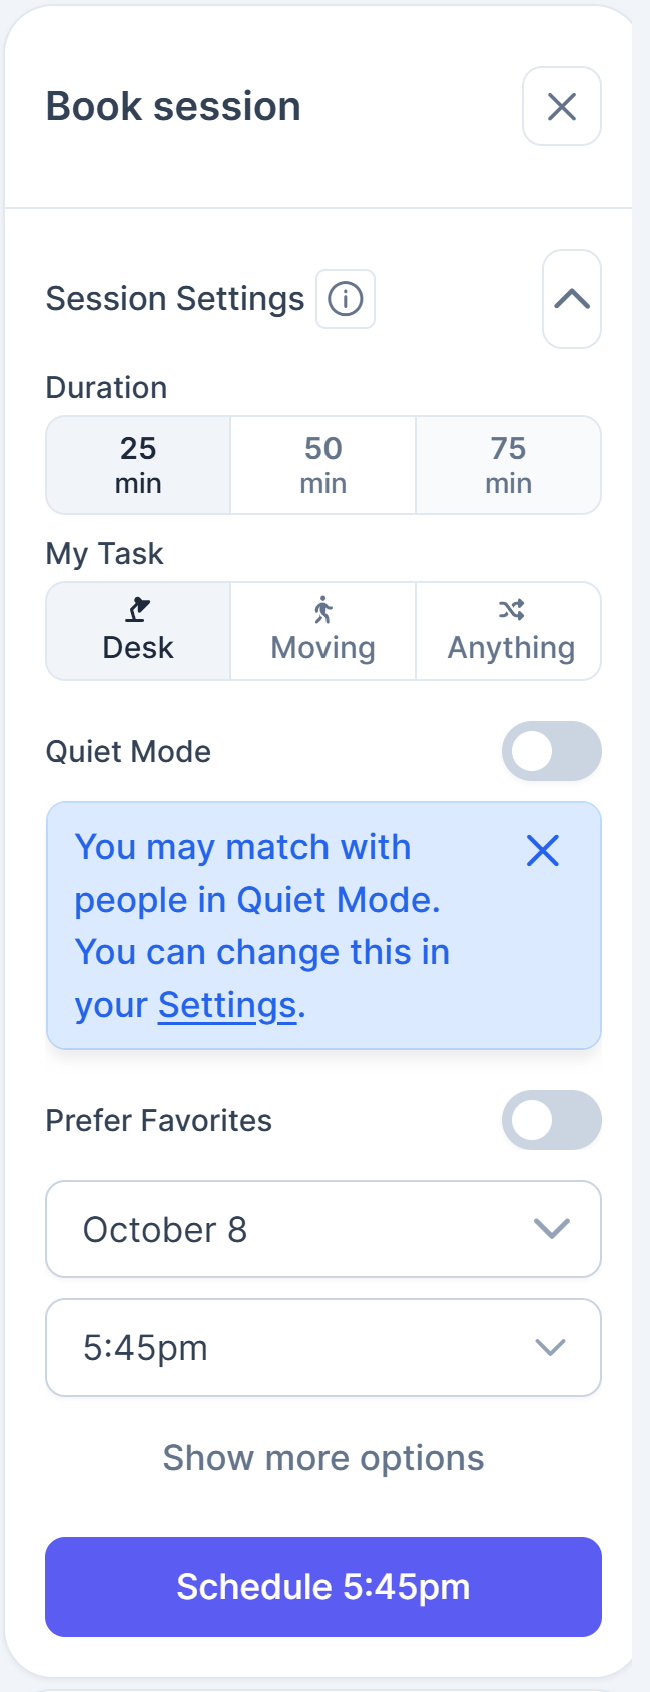
\includegraphics[width=0.3\linewidth]{survey/image/Focusmate/book_session.png}
    \caption{Session booking panel}
    \label{fig:focusmate_book_session}
\end{figure}

\begin{itemize}
    \item To book a session, users follow these steps:
    \begin{enumerate}
        \item Choose the session duration
        \item Specify the task they intend to work on
        \item Choose whether to enable quiet mode
        \item Choose whether to prioritize matching with favorite users
        \item Select a session date using the date bar or calendar
        \item Confirm the booking
    \end{enumerate}
    \item Users can also select a specific date and time directly from the calendar.
    \begin{itemize}
        \item \textbf{Note:} When booking through the calendar, all other session settings remain consistent with the selections made in the session booking panel.
    \end{itemize}
\end{itemize}

\begin{figure}[H]
    \centering
    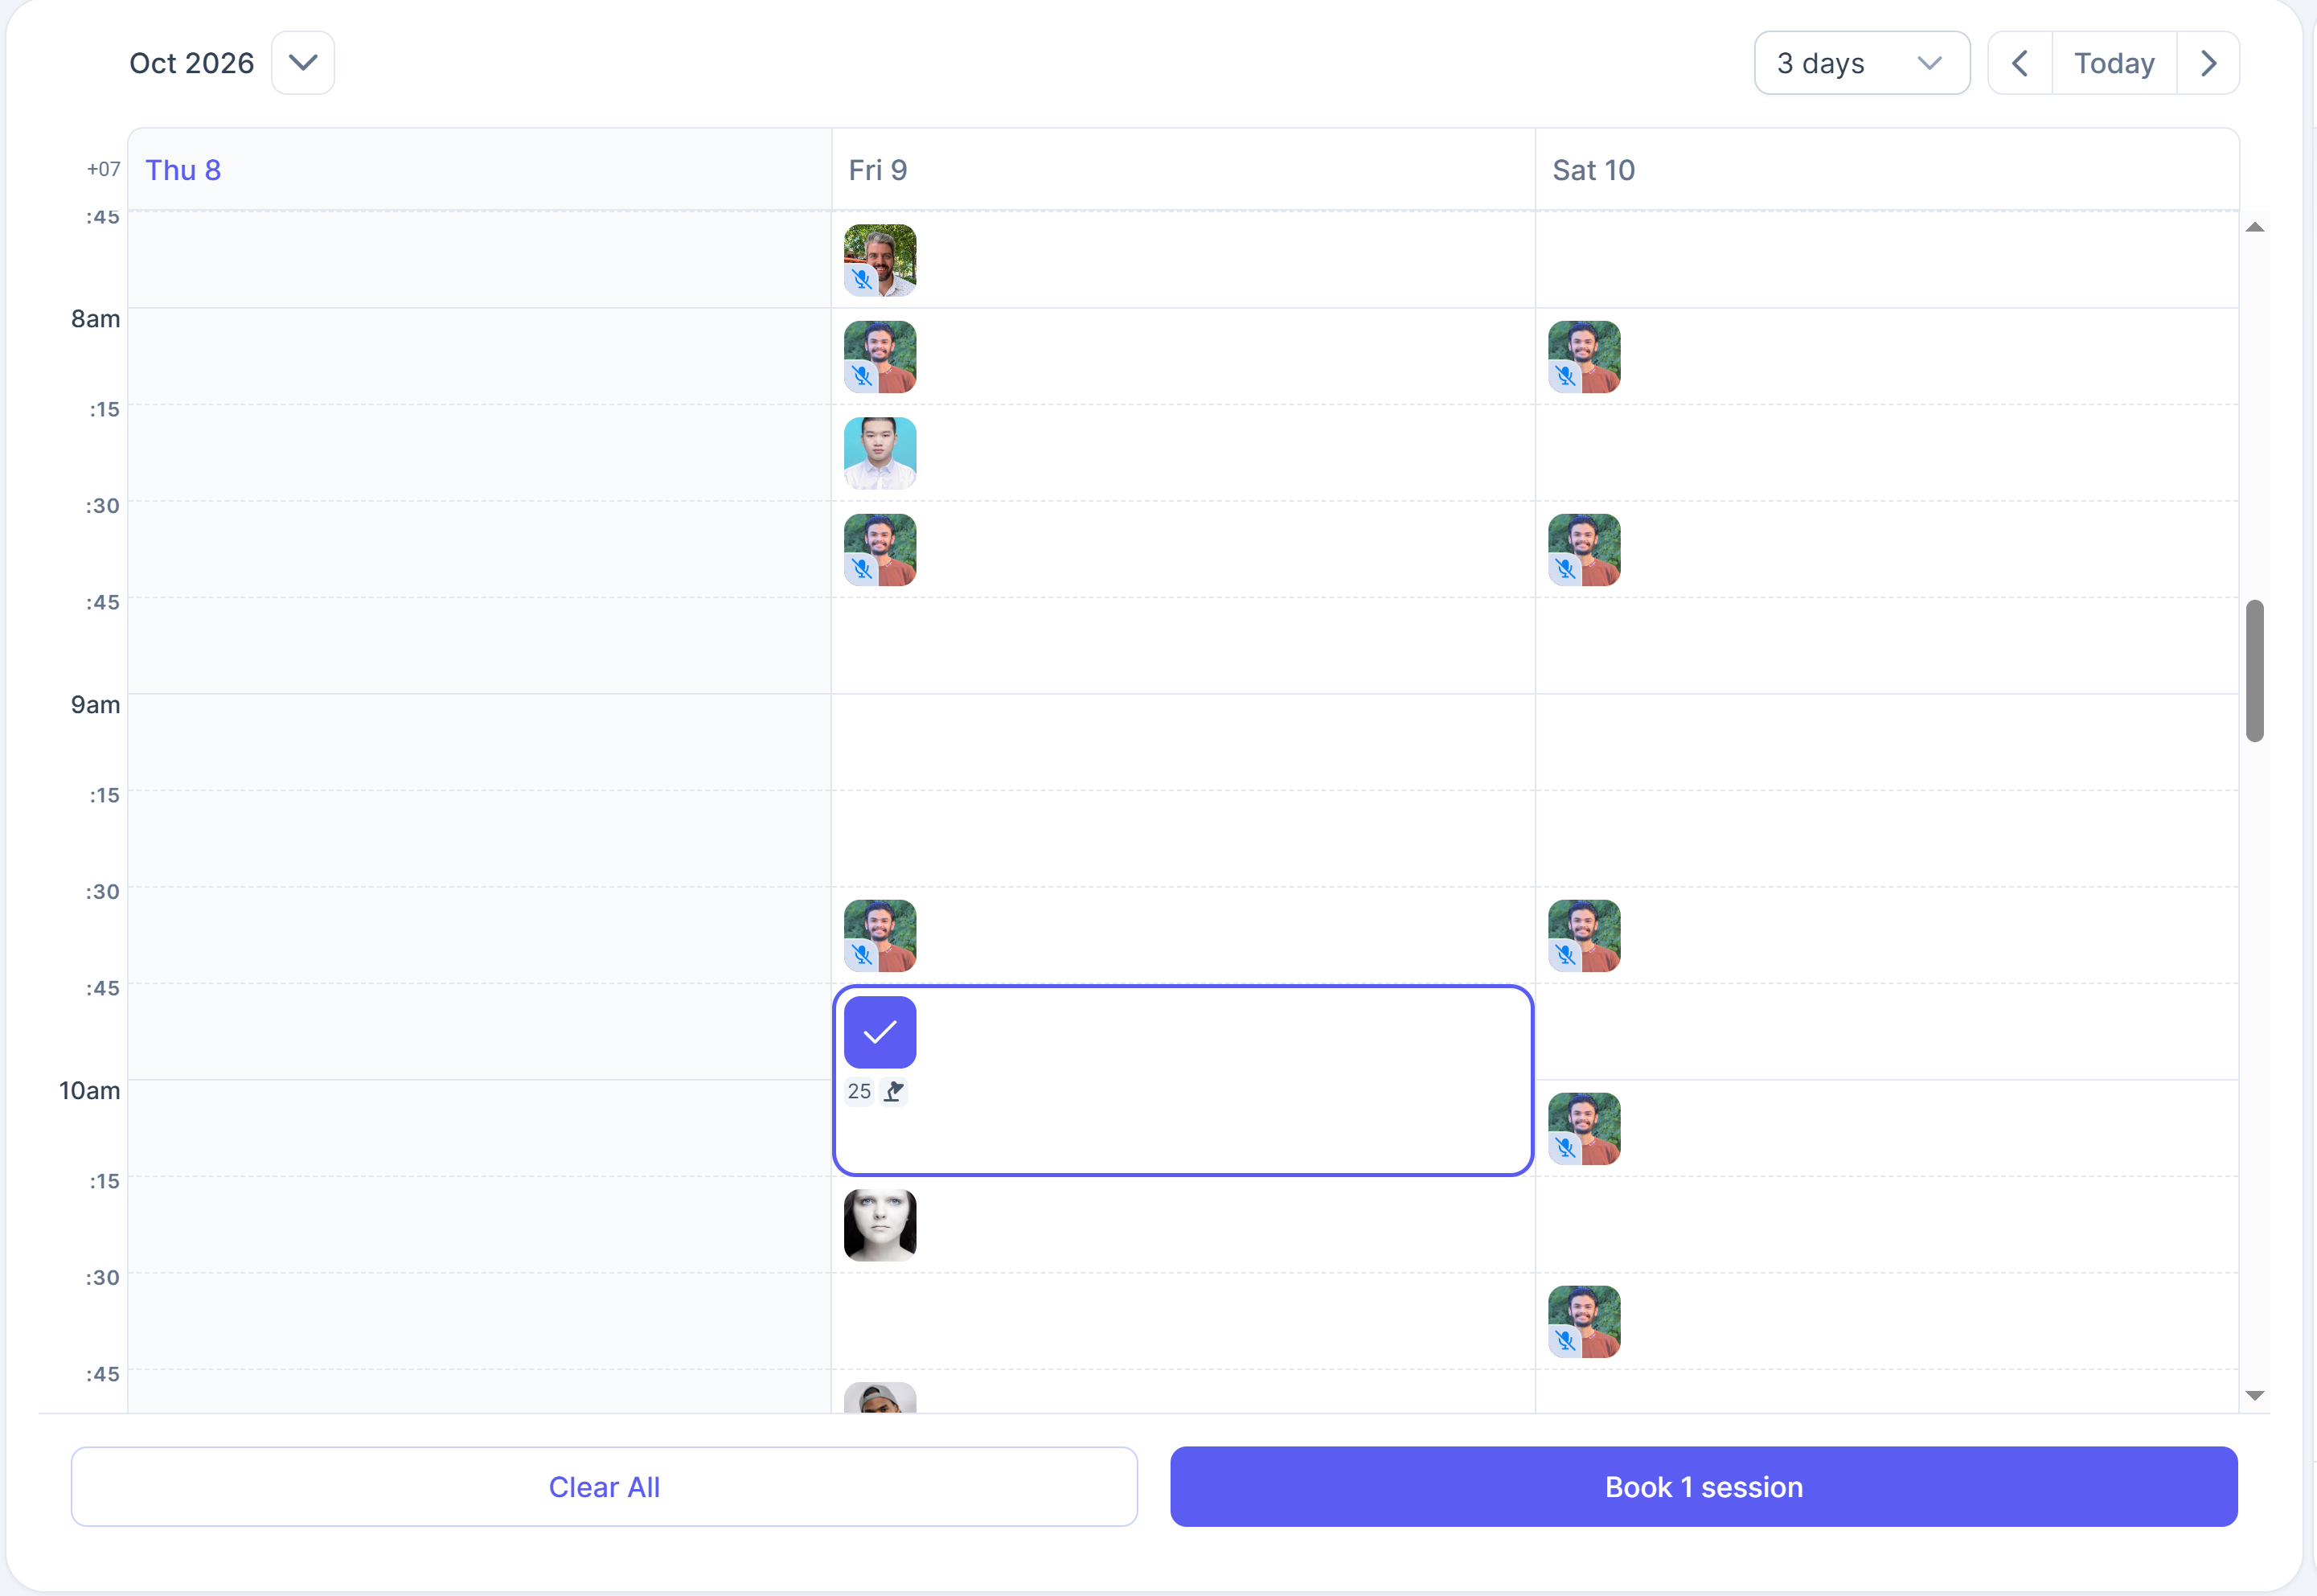
\includegraphics[width=0.6\linewidth]{survey/image/Focusmate/calendar.png}
    \caption{Calendar}
    \label{fig:focusmate_calendar}
\end{figure}

\subsubsection{Joining session:}

\begin{itemize}
    \item Once a session is ready, users can join it:
\end{itemize}

\begin{figure}[H]
    \centering
    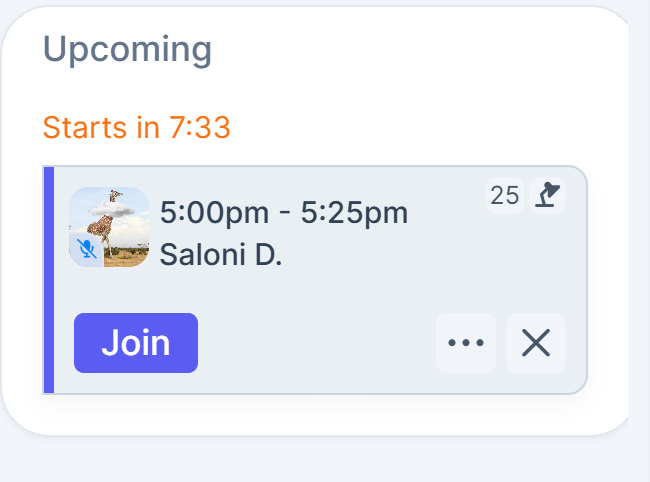
\includegraphics[width=0.6\linewidth]{survey/image/Focusmate/join_session.png}
    \caption{Session joining}
    \label{fig:focusmate_join_session}
\end{figure}

\begin{itemize}
    \item Before joining the video call, users can configure their camera, microphone, speakers, and background effects.
    \begin{itemize}
        \item They can also turn off their camera or mute their microphone as needed.
    \end{itemize}
\end{itemize}

\begin{figure}[H]
    \centering
    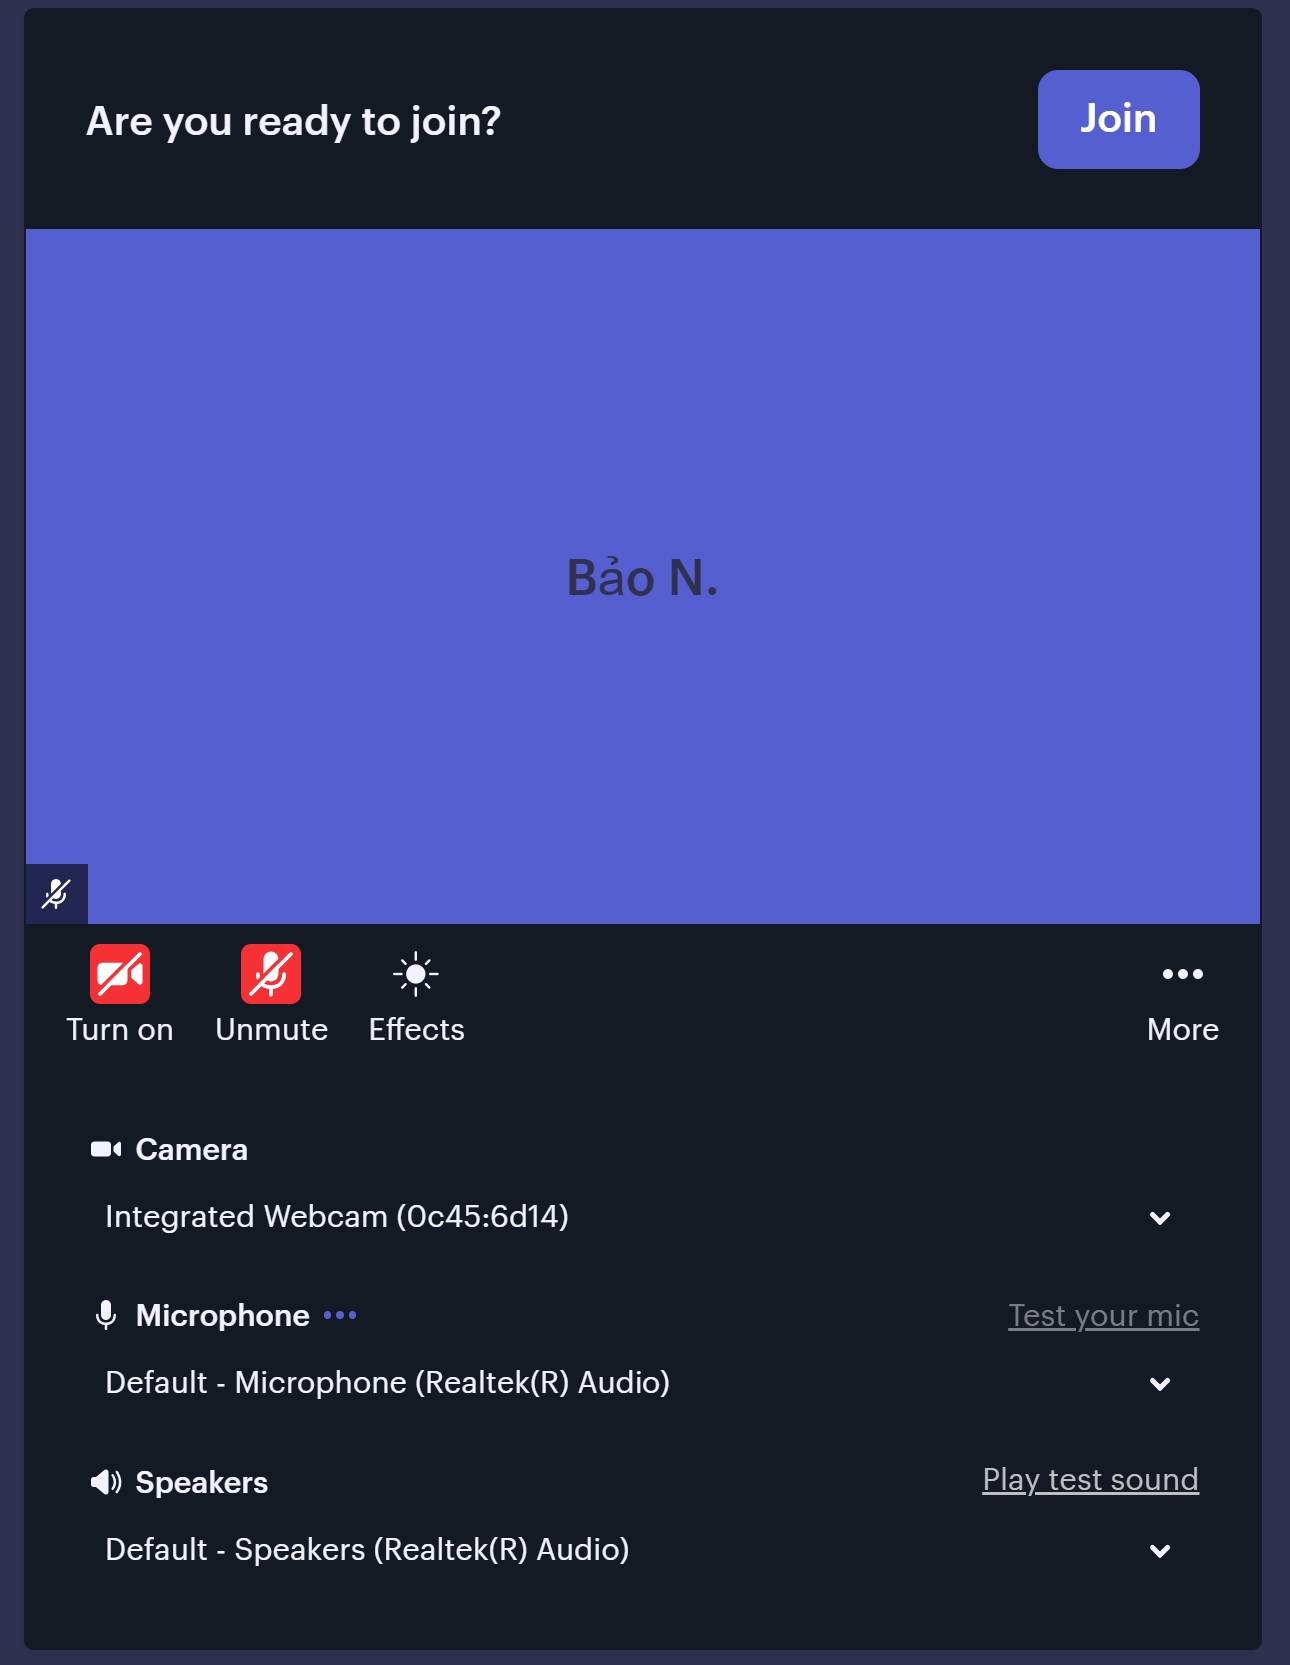
\includegraphics[width=0.7\linewidth]{survey/image/Focusmate/pre_session_setup.png}
    \caption{Pre-session setup}
    \label{fig:focusmate_pre_session_setup}
\end{figure}

\begin{itemize}
    \item After setup, users can join the video call:
\end{itemize}

\begin{figure}[H]
    \centering
    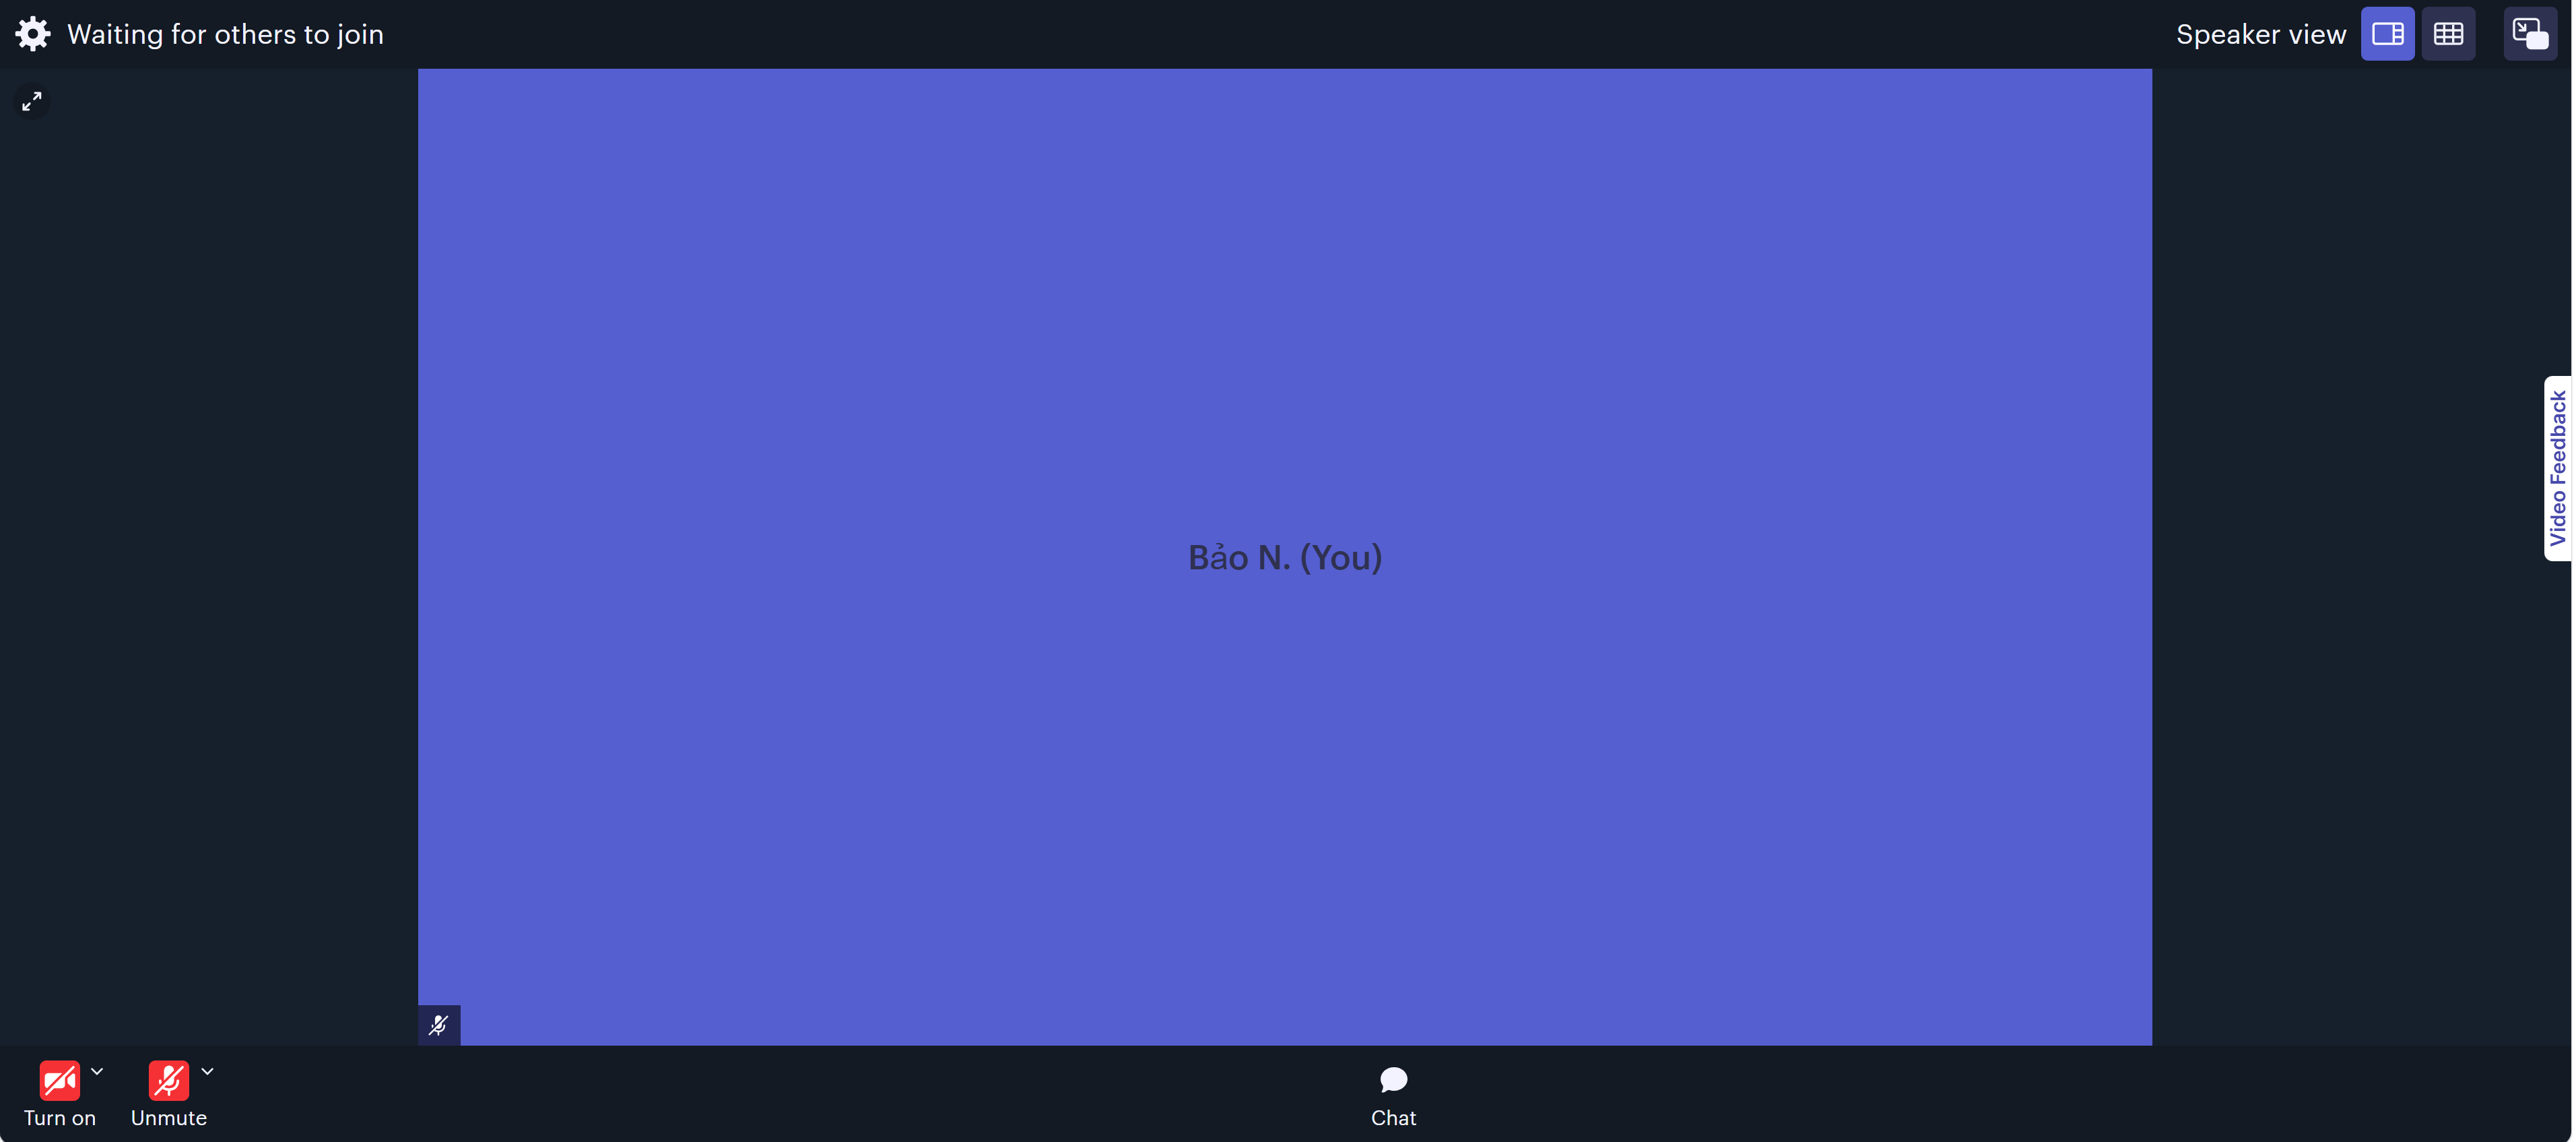
\includegraphics[width=0.7\linewidth]{survey/image/Focusmate/session.png}
    \caption{Session}
    \label{fig:focusmate_session}
\end{figure}

\subsection{Lifeat}

\textbf{Performed by:} [An] | \textbf{Reviewed by:} [Bao] | \textbf{Edited by:} [An]

\begin{itemize}
    \item Lifeat is a platform that focuses on self-studying that allows user to customize their learning space, create, manage and schedule tasks as well as take notes. Besides, it also support learning with friends and study in large meeting with strangers
    \item Link web: \url{https://lifeat.io/}
    \item Lifeat has three modes:
    \begin{itemize}
        \item Focus mode
        \item Explore mode
        \item Plan mode
    \end{itemize}
\end{itemize}

\subsubsection{Focus mode}

\begin{figure}[H]
    \centering
    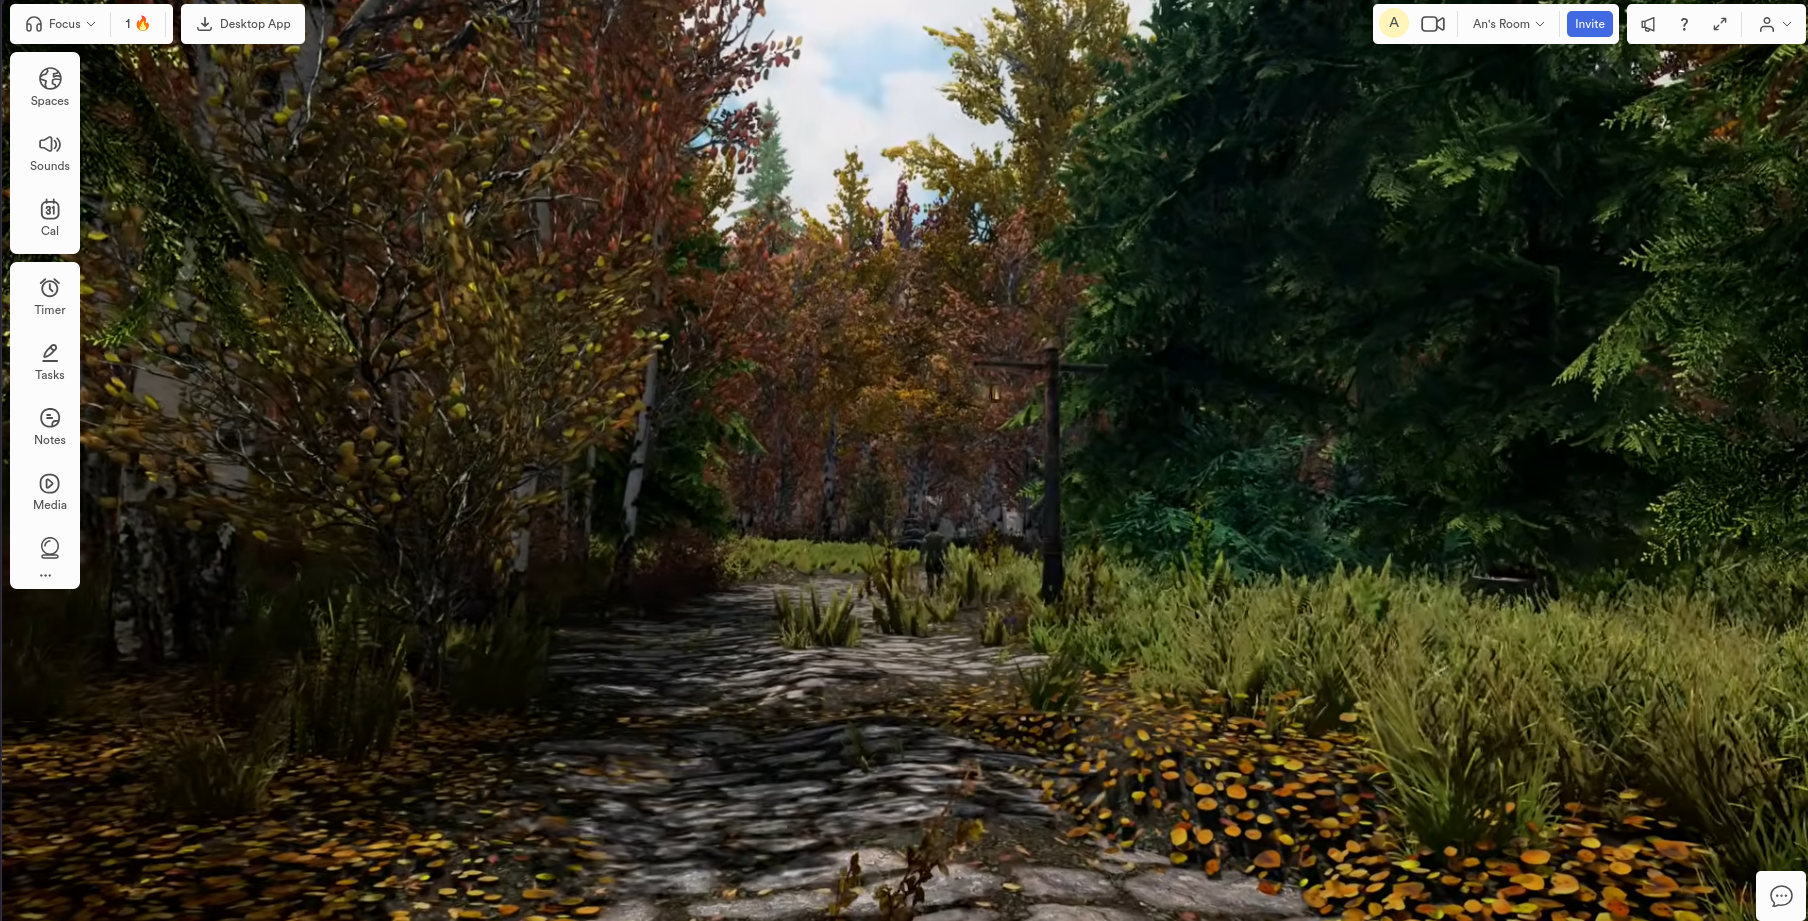
\includegraphics[width=0.85\linewidth]{survey/image/Lifeat/focus_mode_screen.png}
    \caption{Focus mode screen}
    \label{fig:lifeat_focus_mode_screen}
\end{figure}

In this mode, each user enters their own virtual space (as the picture above). In this space, the platform provides following features:

\begin{itemize}
    \item Customize the background:

    \begin{figure}[H]
        \centering
        
\includegraphics[width=0.35\linewidth]{survey/image/Lifeat/space_button.png}
        \caption{Space button}
        \label{fig:lifeat_space_button}
    \end{figure}

    \begin{itemize}
        \item First, click on the spaces icon in the left bar in the focus screen
    \end{itemize}

    \begin{figure}[H]
        \centering
        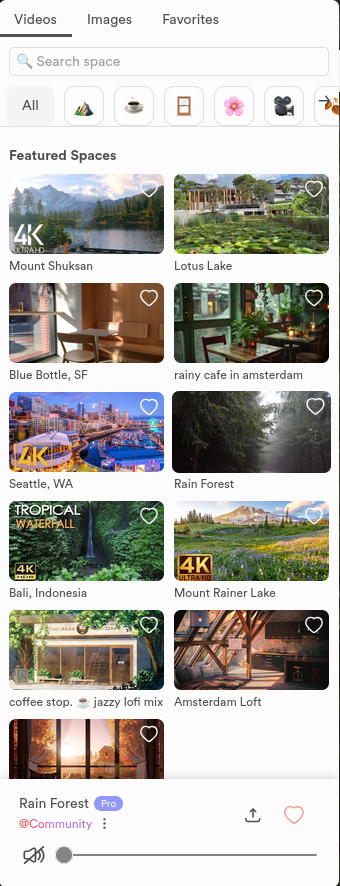
\includegraphics[width=0.4\linewidth]{survey/image/Lifeat/space_window.png}
        \caption{Space Window}
        \label{fig:lifeat_space_window}
    \end{figure}

    \begin{itemize}
        \item There are two kinds of background: Videos background include ambient musics while images do not
    \end{itemize}

    \begin{figure}[H]
        \centering
        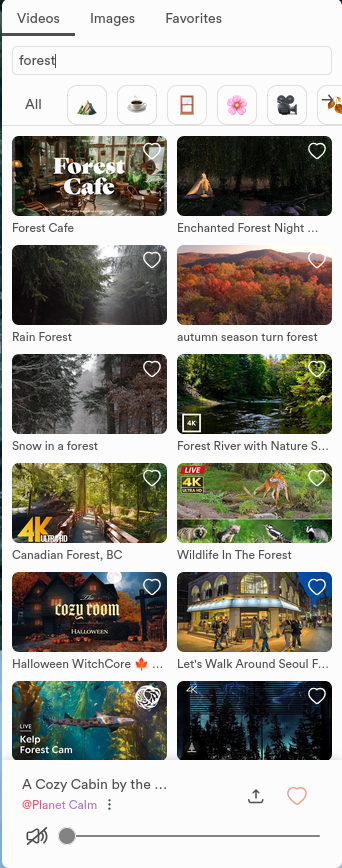
\includegraphics[width=0.4\linewidth]{survey/image/Lifeat/space_search.png}
        \caption{Search spaces}
        \label{fig:lifeat_space_search}
    \end{figure}

    \begin{itemize}
        \item We can search the name of spaces that we want
    \end{itemize}

    \begin{figure}[H]
        \centering
        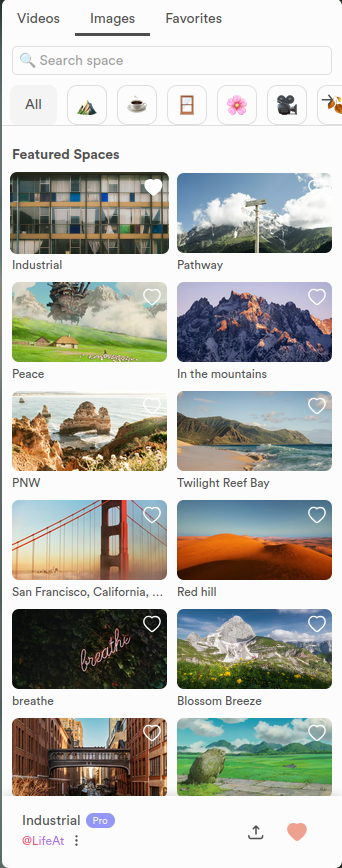
\includegraphics[width=0.5\linewidth]{survey/image/Lifeat/space_favorite.png}
        \caption{Add favorite spaces}
        \label{fig:lifeat_space_favorite}
    \end{figure}

    \begin{figure}[H]
        \centering
        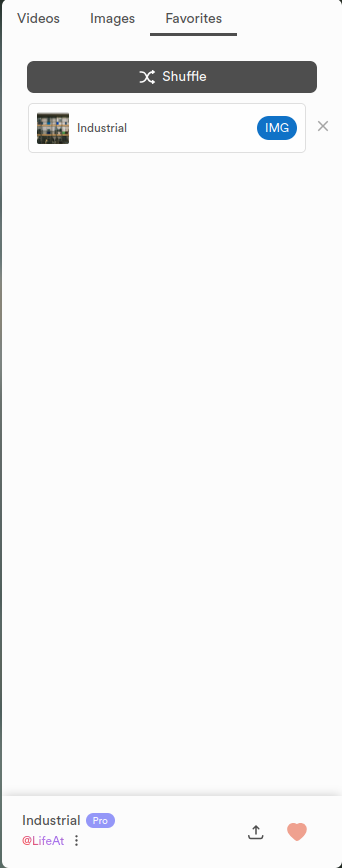
\includegraphics[width=0.5\linewidth]{survey/image/Lifeat/space_favorite_list.png}
        \caption{Watch favorite space}
        \label{fig:lifeat_space_favorite_list}
    \end{figure}

    \begin{itemize}
        \item Besides, if users want to store their favorite background later, they can click the heart icon on the top of background, then it will appear in the Favorites tab
    \end{itemize}

    \item Customize the sound:

    \begin{figure}[H]
        \centering
        
\includegraphics[width=0.35\linewidth]{survey/image/Lifeat/sound_button.png}
        \caption{Sound button}
        \label{fig:lifeat_sound_button}
    \end{figure}

    \begin{itemize}
        \item First, click on the sounds icon in the left bar in the focus screen
    \end{itemize}

    \begin{figure}[H]
        \centering
        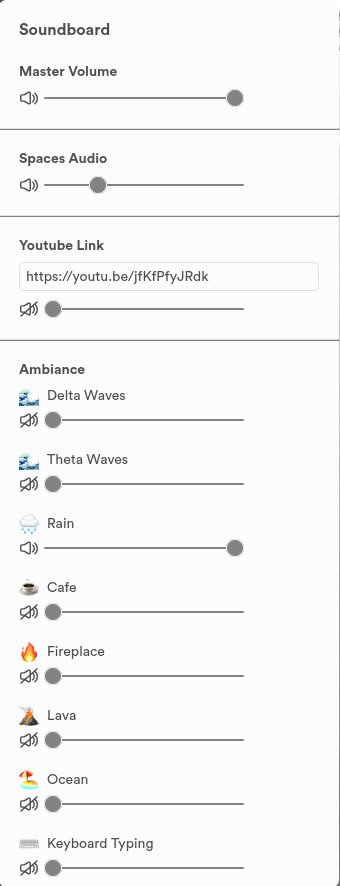
\includegraphics[width=0.4\linewidth]{survey/image/Lifeat/sound_window.png}
        \caption{Sound window}
        \label{fig:lifeat_sound_window}
    \end{figure}

    \begin{itemize}
        \item Then in the sound window, we can:
        \begin{itemize}
            \item Adjust the total volume (master volume)
            \item Adjust the space volume
            \item Insert Youtube music video link and adjust its volume
            \item Choose from the available ambiance sounds and adjust their volumes
        \end{itemize}
    \end{itemize}

    \item Integrate media:

    \begin{figure}[H]
        \centering
        
\includegraphics[width=0.35\linewidth]{survey/image/Lifeat/media_button.png}
        \caption{Media button}
        \label{fig:lifeat_media_button}
    \end{figure}

    \begin{itemize}
        \item First, click on the media icon in the left bar in the focus screen
    \end{itemize}

    \begin{figure}[H]
        \centering
        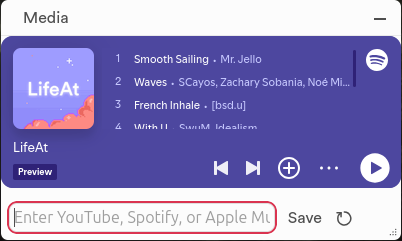
\includegraphics[width=0.6\linewidth]{survey/image/Lifeat/media_window.png}
        \caption{Media window}
        \label{fig:lifeat_media_window}
    \end{figure}

    \begin{figure}[H]
        \centering
        
\includegraphics[width=0.6\linewidth]{survey/image/Lifeat/media_video.png}
        \caption{Media video}
        \label{fig:lifeat_media_video}
    \end{figure}

    \begin{itemize}
        \item Then the media window appears
        \item Insert link Youtube, Spotify or Apple Music to display users' video or playlist
    \end{itemize}

    \item Manage task:

    \begin{figure}[H]
        \centering
        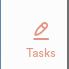
\includegraphics[width=0.35\linewidth]{survey/image/Lifeat/task_button.png}
        \caption{Task button}
        \label{fig:lifeat_task_button}
    \end{figure}

    \begin{itemize}
        \item First, click on the task icon in the left bar in the focus screen
    \end{itemize}

    \begin{figure}[H]
        \centering
        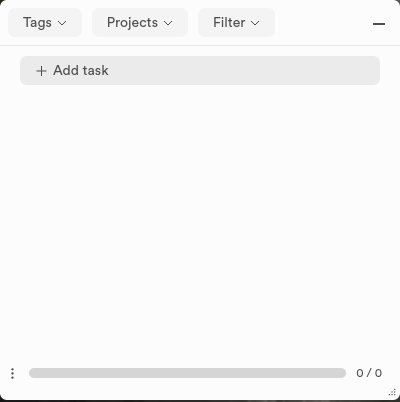
\includegraphics[width=0.6\linewidth]{survey/image/Lifeat/task_window.png}
        \caption{Task window}
        \label{fig:lifeat_task_window}
    \end{figure}

    \begin{itemize}
        \item The task window then appears
    \end{itemize}

    \begin{figure}[H]
        \centering
        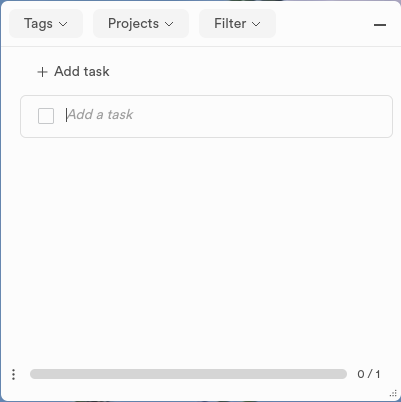
\includegraphics[width=0.5\linewidth]{survey/image/Lifeat/task_create.png}
        \caption{Create a task}
        \label{fig:lifeat_task_create}
    \end{figure}

    \begin{itemize}
        \item To create a task, click on add task button. A new task appears and users give it a name
    \end{itemize}

    \begin{figure}[H]
        \centering
        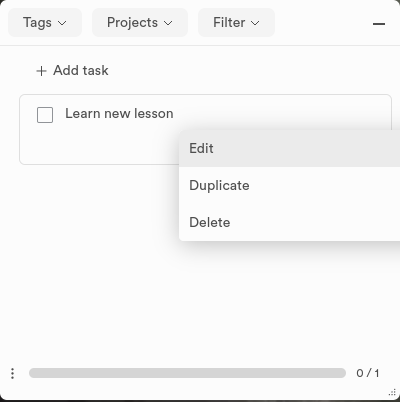
\includegraphics[width=0.5\linewidth]{survey/image/Lifeat/task_edit.png}
        \caption{Edit a task}
        \label{fig:lifeat_task_edit}
    \end{figure}

    \begin{figure}[H]
        \centering
        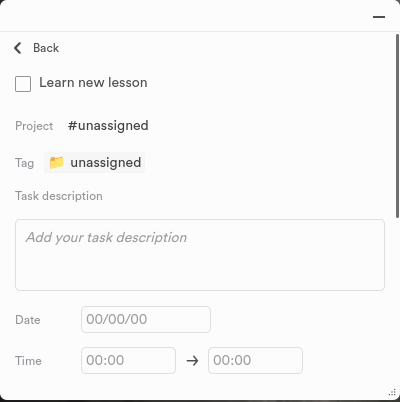
\includegraphics[width=0.5\linewidth]{survey/image/Lifeat/task_info1.png}
        \caption{Provide further information for a task 1}
        \label{fig:lifeat_task_info1}
    \end{figure}

    \begin{figure}[H]
        \centering
        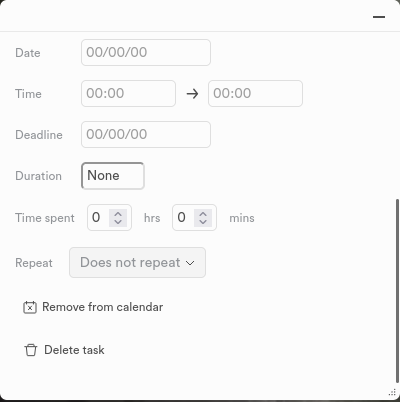
\includegraphics[width=0.5\linewidth]{survey/image/Lifeat/task_info2.png}
        \caption{Provide further information for a task 2}
        \label{fig:lifeat_task_info2}
    \end{figure}

    \begin{itemize}
        \item To provide additional information for a task, we can do following steps:
        \begin{itemize}
            \item Right-click the task to display the option
            \item Choose edit option
            \item Provide the necessary information for the task
        \end{itemize}
    \end{itemize}

    \begin{figure}[H]
        \centering
        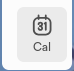
\includegraphics[width=0.35\linewidth]{survey/image/Lifeat/calendar_button.png}
        \caption{Calendar button}
        \label{fig:lifeat_calendar_button}
    \end{figure}

    \begin{figure}[H]
        \centering
        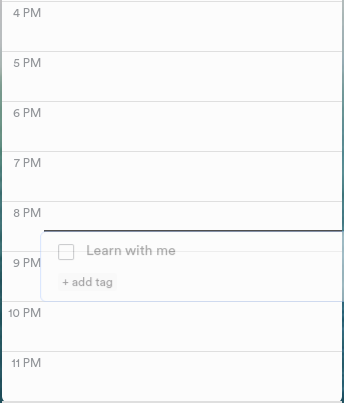
\includegraphics[width=0.6\linewidth]{survey/image/Lifeat/task_schedule.png}
        \caption{Schedule a task}
        \label{fig:lifeat_task_schedule}
    \end{figure}

    \begin{itemize}
        \item Beside, setting time information for a task, users can schedule it by drag the task into the Calendar window after clicking calendar button
    \end{itemize}

    \item Countdown timer

    \begin{figure}[H]
        \centering
        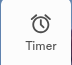
\includegraphics[width=0.35\linewidth]{survey/image/Lifeat/timer_button.png}
        \caption{Timer button}
        \label{fig:lifeat_timer_button}
    \end{figure}

    \begin{itemize}
        \item First, click on the timer icon in the left bar in the focus screen. users have three types of countdown timers: Pomodoro (20 min), Short break(5 min), Long break (15 min) and three mode: Personal, Group, Task
    \end{itemize}

    \begin{figure}[H]
        \centering
        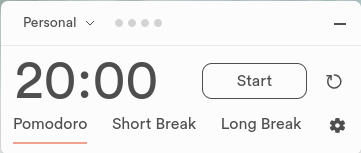
\includegraphics[width=0.6\linewidth]{survey/image/Lifeat/timer_personal.png}
        \caption{Personal timer}
        \label{fig:lifeat_timer_personal}
    \end{figure}

    \begin{itemize}
        \item The personal timer is designed for individual use without being associated with a specific task. This mode is suitable for users who want to apply the Pomodoro Technique.
    \end{itemize}

    \begin{figure}[H]
        \centering
        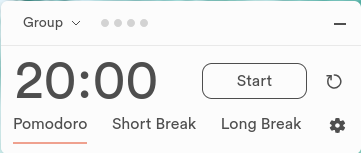
\includegraphics[width=0.6\linewidth]{survey/image/Lifeat/timer_group.png}
        \caption{Group timer}
        \label{fig:lifeat_timer_group}
    \end{figure}

    \begin{itemize}
        \item This mode is used when users learn with other people. When it is created, all people in the room can see this timer
    \end{itemize}

    \begin{figure}[H]
        \centering
        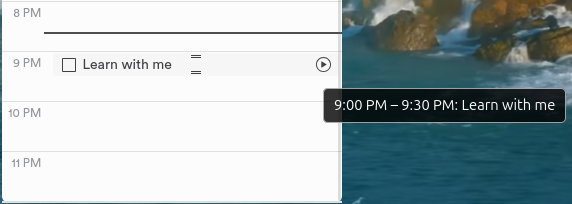
\includegraphics[width=0.5\linewidth]{survey/image/Lifeat/timer_task_play.png}
        \caption{Task timer play}
        \label{fig:lifeat_timer_task_play}
    \end{figure}

    \begin{figure}[H]
        \centering
        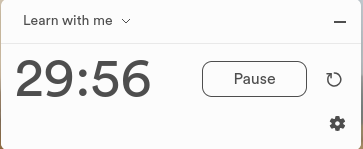
\includegraphics[width=0.6\linewidth]{survey/image/Lifeat/timer_task.png}
        \caption{Task timer countdown}
        \label{fig:lifeat_timer_task}
    \end{figure}

    \begin{itemize}
        \item To start a timer for a specific task, users can click the play button on the task in the calendar window.
        \item The task-specific countdown timer then appears.
    \end{itemize}

    \item Take notes

    \begin{figure}[H]
        \centering
        
\includegraphics[width=0.35\linewidth]{survey/image/Lifeat/notes_button.png}
        \caption{Notes button}
        \label{fig:lifeat_notes_button}
    \end{figure}

    \begin{itemize}
        \item First, click on the notes icon in the left bar in the focus screen.
    \end{itemize}

    \begin{figure}[H]
        \centering
        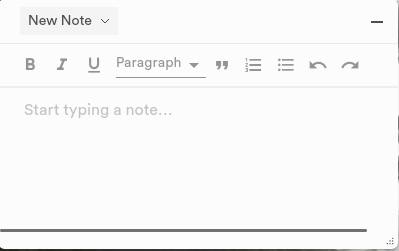
\includegraphics[width=0.6\linewidth]{survey/image/Lifeat/notes_window.png}
        \caption{Notes window}
        \label{fig:lifeat_notes_window}
    \end{figure}

    \begin{itemize}
        \item Then the Notes window appears, users can write note and apply formatting the note such as bold, underline, ... by the function bar on the top
    \end{itemize}

    \begin{figure}[H]
        \centering
        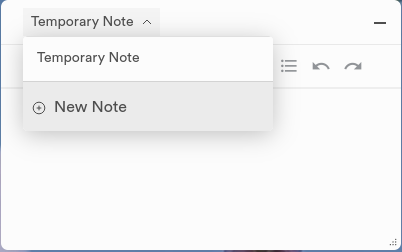
\includegraphics[width=0.5\linewidth]{survey/image/Lifeat/notes_create.png}
        \caption{Create a new note}
        \label{fig:lifeat_notes_create}
    \end{figure}

    \begin{itemize}
        \item Users can create a new note by clicking in the top-left corner of the Notes window then, it will display a panel which has New Note button
    \end{itemize}

    \item Learning with friends

    \begin{figure}[H]
        \centering
        
\includegraphics[width=0.35\linewidth]{survey/image/Lifeat/invite_button.png}
        \caption{Invite button}
        \label{fig:lifeat_invite_button}
    \end{figure}

    \begin{itemize}
        \item First, click the invite button on the top right corner of the focus screen button
    \end{itemize}

    \begin{figure}[H]
        \centering
        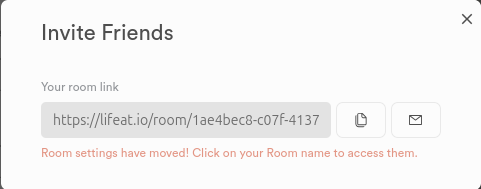
\includegraphics[width=0.6\linewidth]{survey/image/Lifeat/invite_friend.png}
        \caption{Link to invite}
        \label{fig:lifeat_invite_friend}
    \end{figure}

    \begin{itemize}
        \item After that, an invitation window appears, users can send this link to their friend to invite them to join their virtual space
    \end{itemize}

    \begin{figure}[H]
        \centering
        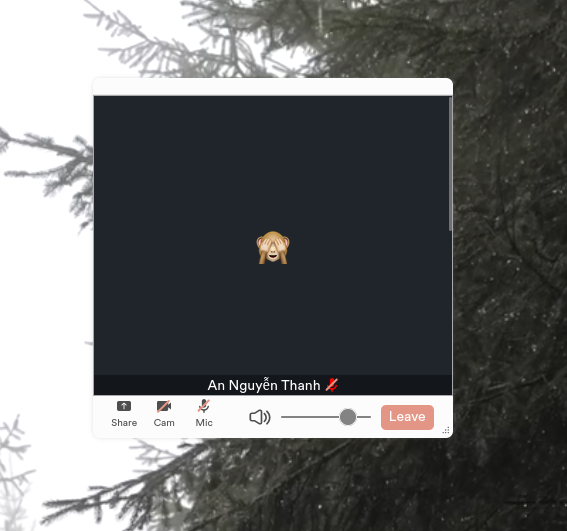
\includegraphics[width=0.7\linewidth]{survey/image/Lifeat/video_call.png}
        \caption{Video call with friends}
        \label{fig:lifeat_video_call}
    \end{figure}

    \begin{itemize}
        \item When their friend join the room, users can make video call by click on the camera icon on the invite bar. The platform also allows users to share their screens
    \end{itemize}

    \begin{figure}[H]
        \centering
        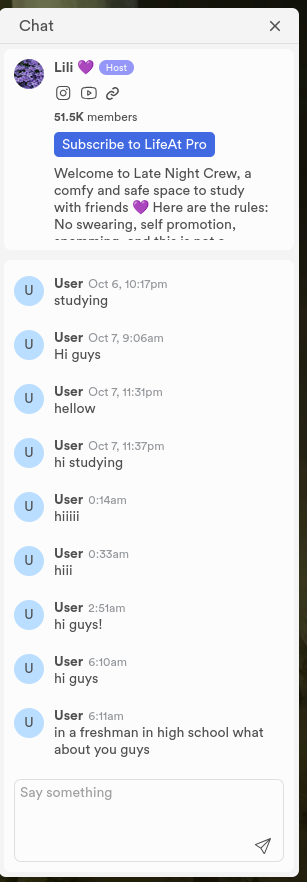
\includegraphics[width=0.4\linewidth]{survey/image/Lifeat/chat.png}
        \caption{Chat with friends}
        \label{fig:lifeat_chat}
    \end{figure}

    \begin{itemize}
        \item Users can send text messages to other participants in the room
    \end{itemize}
\end{itemize}

\subsubsection{Explore mode}

\begin{figure}[H]
    \centering
    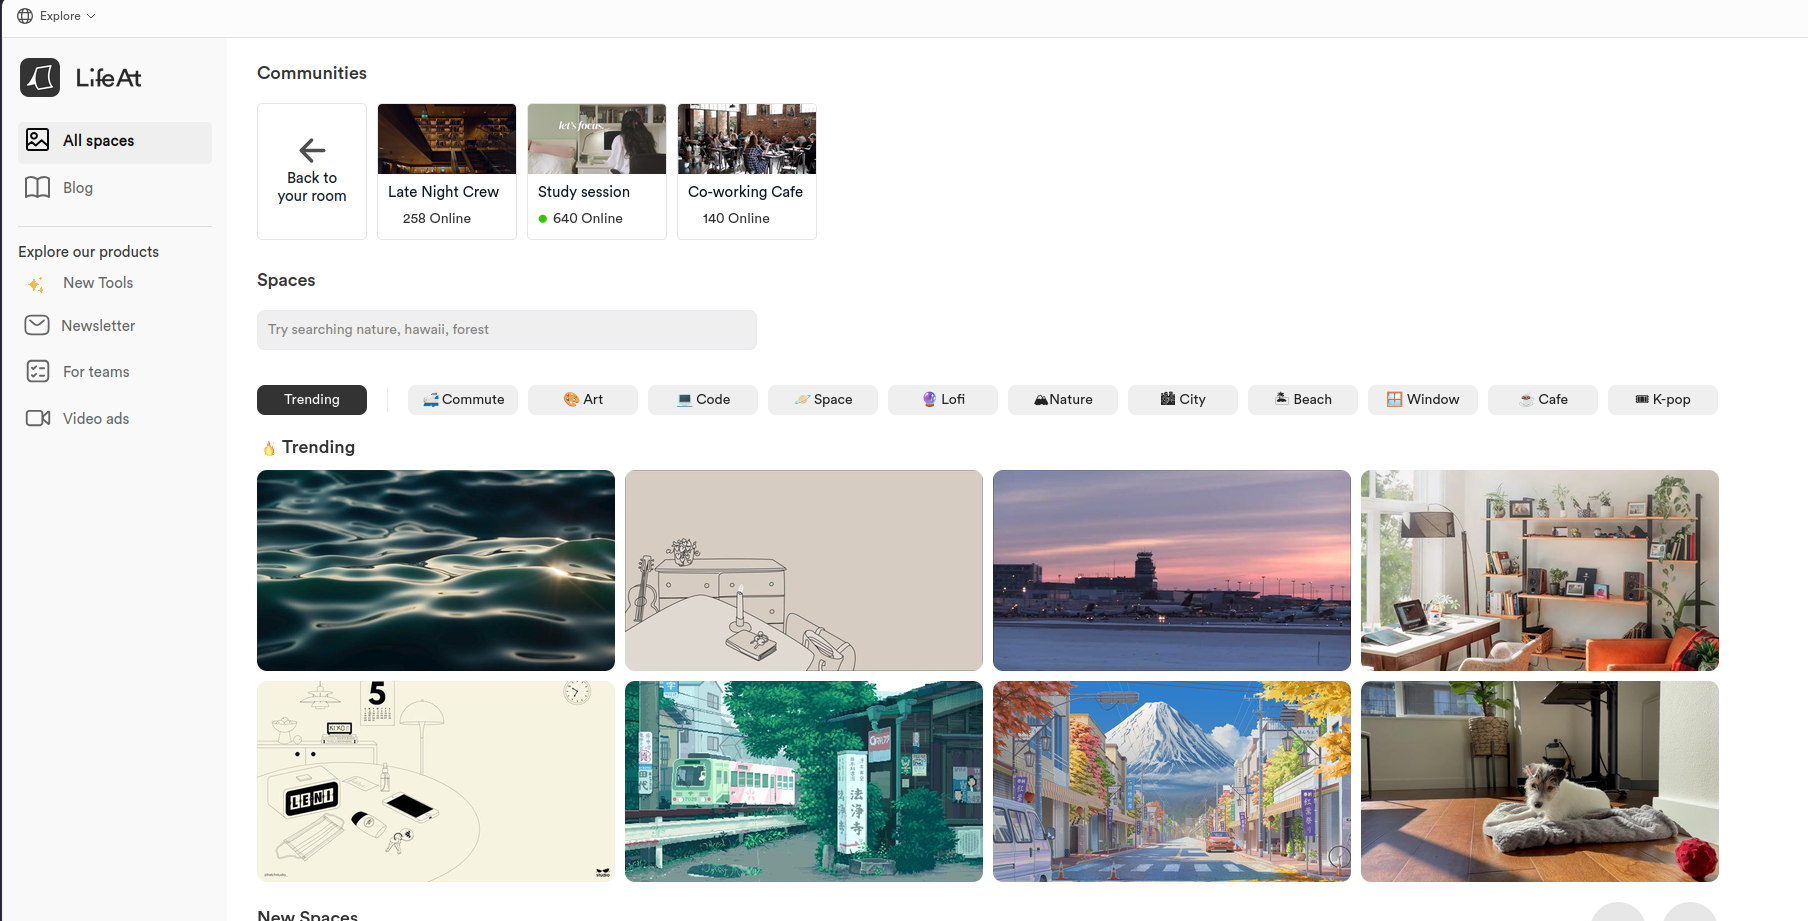
\includegraphics[width=0.85\linewidth]{survey/image/Lifeat/explore_mode_screen.png}
    \caption{Explore mode screen}
    \label{fig:lifeat_explore_mode_screen}
\end{figure}

In this mode, instead of self-studying or with friends, users can study with strangers

The platform provides communities that offer shared virtual study spaces similar to those in Focus mode.

\subsubsection{Plan mode}

\begin{figure}[H]
    \centering
    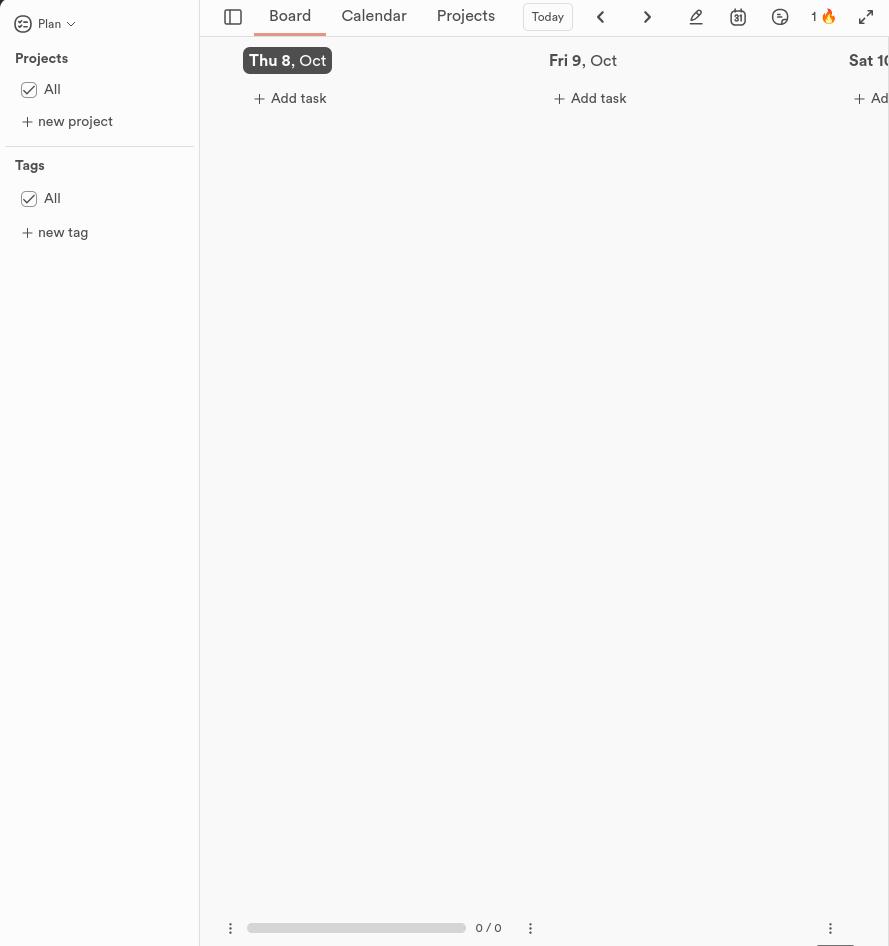
\includegraphics[width=0.85\linewidth]{survey/image/Lifeat/plan_mode_screen.png}
    \caption{Plan mode screen}
    \label{fig:lifeat_plan_mode_screen}
\end{figure}

In this mode, users can create and manage tasks, similar to the functionality available in Focus mode. Moreover, they can create and manage task in a project.

\begin{itemize}
    \item Create a project:

    \begin{figure}[H]
        \centering
        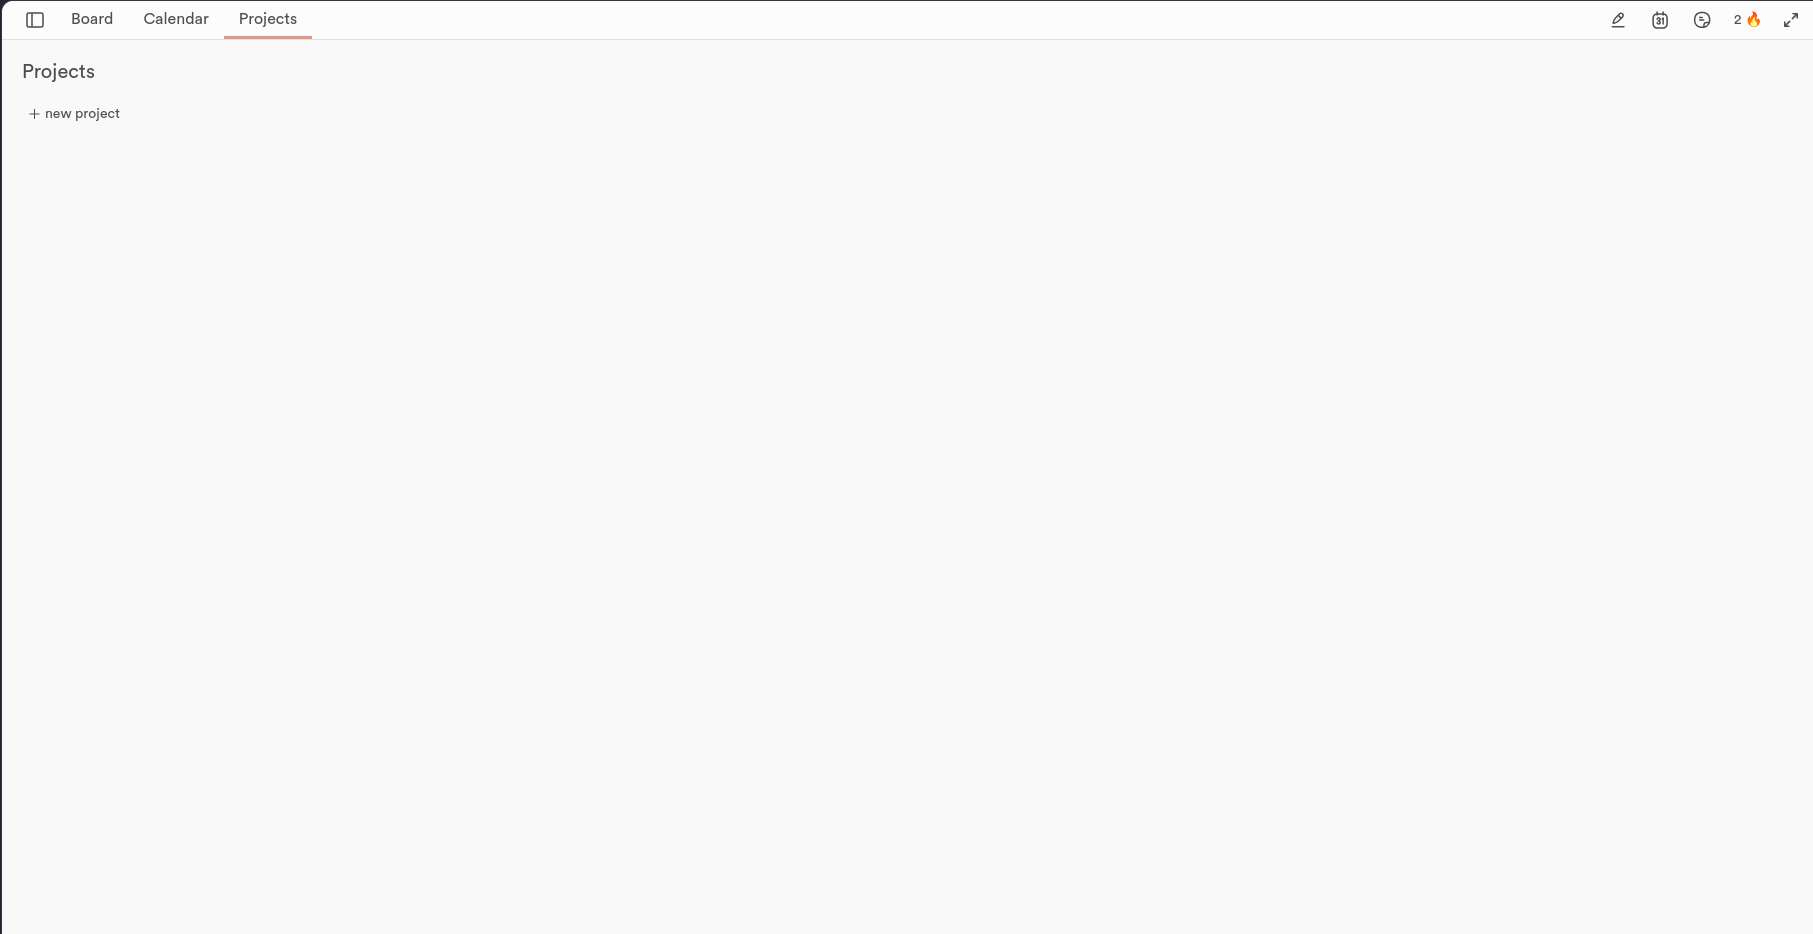
\includegraphics[width=0.6\linewidth]{survey/image/Lifeat/plan_project.png}
        \caption{Project tab}
        \label{fig:lifeat_plan_project}
    \end{figure}

    \begin{itemize}
        \item Click on the project tab on the Plan mode to see the Project tab
    \end{itemize}

    \begin{figure}[H]
        \centering
        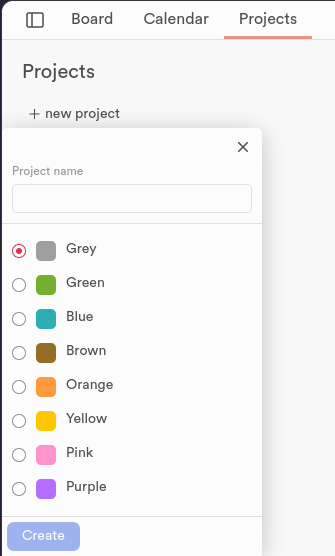
\includegraphics[width=0.5\linewidth]{survey/image/Lifeat/project_create.png}
        \caption{Create a project}
        \label{fig:lifeat_project_create}
    \end{figure}

    \begin{itemize}
        \item Click create project button to add a new one
    \end{itemize}

    \begin{figure}[H]
        \centering
        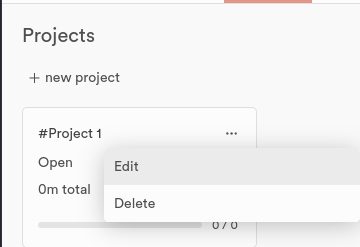
\includegraphics[width=0.5\linewidth]{survey/image/Lifeat/project_edit.png}
        \caption{Edit a project}
        \label{fig:lifeat_project_edit}
    \end{figure}

    \begin{figure}[H]
        \centering
        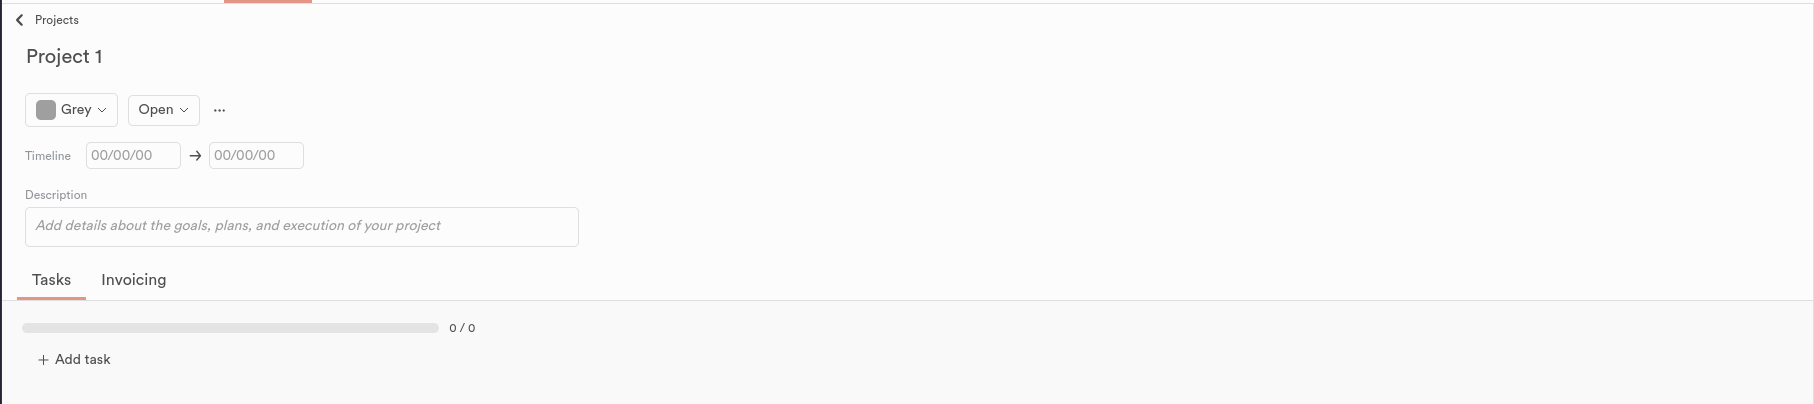
\includegraphics[width=0.6\linewidth]{survey/image/Lifeat/project_manager.png}
        \caption{Project manager tab}
        \label{fig:lifeat_project_manager}
    \end{figure}

    \begin{itemize}
        \item To add tasks, edit the description, or perform other actions, users can right-click the project then press edit to display the project manager tab
        \item Then they can adjust the information, manage task similar to focus mode
    \end{itemize}
\end{itemize}

\subsection{Summary}

Focusmate and Lifeat are productivity platforms that help users maintain focus and improve their productivity through different approaches. Focusmate emphasizes virtual coworking and personal accountability, whereas Lifeat provides a customizable study environment with task management, scheduling, and collaborative learning features.

Although Focusmate and Lifeat take different approaches to productivity, they share several important characteristics:

\begin{itemize}
    \item Focus-oriented experiences: Both platforms help users concentrate on their work or study activities
    \item Collaborative learning and working: Both support interaction with other people. Focusmate matches users for scheduled coworking sessions, while Lifeat enables users to study with friends or participate in shared study spaces
    \item Flexible work sessions: Both support structured periods of focused work, although their implementations differ. Focusmate uses predefined session durations, while Lifeat provides configurable countdown timers and different timer modes
    \item User-controlled experiences: Both allow users to configure aspects of their experience. Focusmate provides session preferences, while Lifeat offers customizable backgrounds, sounds, and media.
    \item Support for productivity routines: Both provide mechanisms that help users organize their time and maintain focus, although Lifeat offers more extensive task planning and scheduling functionality.
\end{itemize}

\subsubsection{What Our Proposed App Will Do Differently or Better}

Based on the available features of Focusmate and Lifeat, we observe and adapt the following features to our application:

\begin{itemize}
    \item \textbf{Quiet Mode and Communication:}
    \begin{itemize}
        \item Enhance Quiet Mode by allowing students to send hand-wave requests to initiate conversations without unnecessarily interrupting others.
        \item Require recipients to accept interaction requests before communication begins, giving students greater control over their focus and availability.
    \end{itemize}
    \item \textbf{Learning Room Structure:}
    \begin{itemize}
        \item Enhance existing virtual study spaces by supporting multiple tables within a shared room, allowing students to study independently or alongside others.
        \item Allow students to create dynamic groups with customizable sizes, each with independent voice communication, text chat, and collaboration tools.
    \end{itemize}
    \item \textbf{Friend System:}
    \begin{itemize}
        \item Extend the existing favorite-user and friend-invitation features into a persistent friend system that supports sending, accepting, and managing friend requests.
        \item Allow students to create messaging groups and share learning documents, supporting long-term collaboration beyond individual study sessions.
    \end{itemize}
    \item \textbf{Task Planning and Scheduling:}
    \begin{itemize}
        \item Extend existing task management and scheduling features by integrating study plans with learning room creation and organization.
        \item Allow students to create rooms around specific subjects, tasks, or schedules, helping them coordinate collaborative learning activities more effectively.
    \end{itemize}
\end{itemize}

Moreover, we propose the following new features to better support our application's purpose:

\begin{itemize}
    \item \textbf{University-based Communities:}
    \begin{itemize}
        \item Organize students into university-specific communities, restricting public learning rooms to eligible students from participating universities.
        \item Allow students to create private rooms for their own study groups, providing greater control over room access.
    \end{itemize}
    \item \textbf{Learning Assistance:}
    \begin{itemize}
        \item Introduce voice-based help requests so students can seek assistance from other learners when encountering difficult concepts.
        \item Provide a discussion forum where students can post questions, share problems, and receive answers asynchronously, supporting peer-to-peer learning without requiring real-time interaction.
    \end{itemize}
    \item \textbf{Study Partner Recommendations:}
    \begin{itemize}
        \item Recommend potential study partners based on similar learning interests and study schedules.
        \item Allow room owners to review and approve participation requests from recommended learners, providing greater control over group composition.
    \end{itemize}
\end{itemize}

\pagebreak
% ============================================================
% SECTION 3: CONTRACT
% ============================================================
\section{Team Contract}

\subsection{1. Team Members and Roles}

\textbf{Performed by:} [Tuan] | \textbf{Reviewed by:} [An] | \textbf{Edited by:} [An]

\begin{table}[H]
\centering\footnotesize
\setlength{\tabcolsep}{3pt}
\begin{tabular}{|c|c|l|l|l|}
\hline
No. & Student ID & Full Name & Email & Primary Role \\
\hline
1 & 24125024 & Nguyễn Thanh An & ntan2419@apcs.fitus.edu.vn & Front-end Developer \\
\hline
2 & 24125025 & Nguyễn Chí Bảo & ncbao2434@apcs.fitus.edu.vn & Tester + AI Developer \\
\hline
3 & 24125026 & Trần Nguyễn Khánh Bình & tnkbinh2414@apcs.fitus.edu.vn & UI Designer \\
\hline
4 & 24125048 & Trần Cảnh Anh Tuấn & tcatuan2413@apcs.fitus.edu.vn & Database Manager \\
\hline
5 & 24125100 & Nguyễn Lê Quốc Huy & nlqhuy2414@apcs.fitus.edu.vn & Back-end Developer \\
\hline
\end{tabular}
\end{table}

All members are full-stack engineers. A primary role identifies an area of leadership and responsibility; it does not limit a member's participation in other areas. Every member participates in requirements, design, implementation, testing, documentation, and review.

\subsection{2. Communication Plan}

\textbf{Performed by:} [Tuan] | \textbf{Reviewed by:} [An] | \textbf{Edited by:} [An]**

\begin{table}[H]
\centering
\begin{tabular}{|l|p{0.55\linewidth}|}
\hline
Tool & Purpose \\
\hline
Moodle & Official assignment submission, course announcements and discussion \\
\hline
Messenger, Discord & Team communication \\
\hline
Jira & Task management \\
\hline
GitHub & Source code and documentation \\
\hline
\end{tabular}
\end{table}

\begin{itemize}
    \item Members normally respond to non-urgent messages within \textbf{12 hours}.
    \item Urgent issues should be acknowledged as soon as reasonably possible, preferably within \textbf{2 hours during normal availability}.
    \item Members should notify the team when they will be unavailable for an extended period.
    \item Important decisions and action items are recorded in the project workspace.
    \item Conflicts follow the process defined in Section 7.
\end{itemize}

\subsection{3. Work Schedule and Scrum Process}

\textbf{Performed by:} [Tuan] | \textbf{Reviewed by:} [An] | \textbf{Edited by:} [An]

The team follows the Scrum process. Each Sprint includes:

\begin{itemize}
    \item \textbf{1 Sprint Planning meeting}
    \item \textbf{2 Scrum meetings}
    \item \textbf{1 Sprint Review meeting}
\end{itemize}

Meeting format follows the course \textbf{WeeklyReports} guidelines.

\subsubsection{Task Management}

Every project-related task must be recorded, including coding, testing, documentation, research, and self-training tasks.

Each task:

\begin{itemize}
    \item Is assigned to \textbf{exactly one} team member.
    \item Has a creation date, assignment date, and completion date.
    \item Is created and assigned \textbf{before work begins}.
    \item Is marked complete only when the work is actually finished.
\end{itemize}

\begin{figure}[htbp]
    \centering
    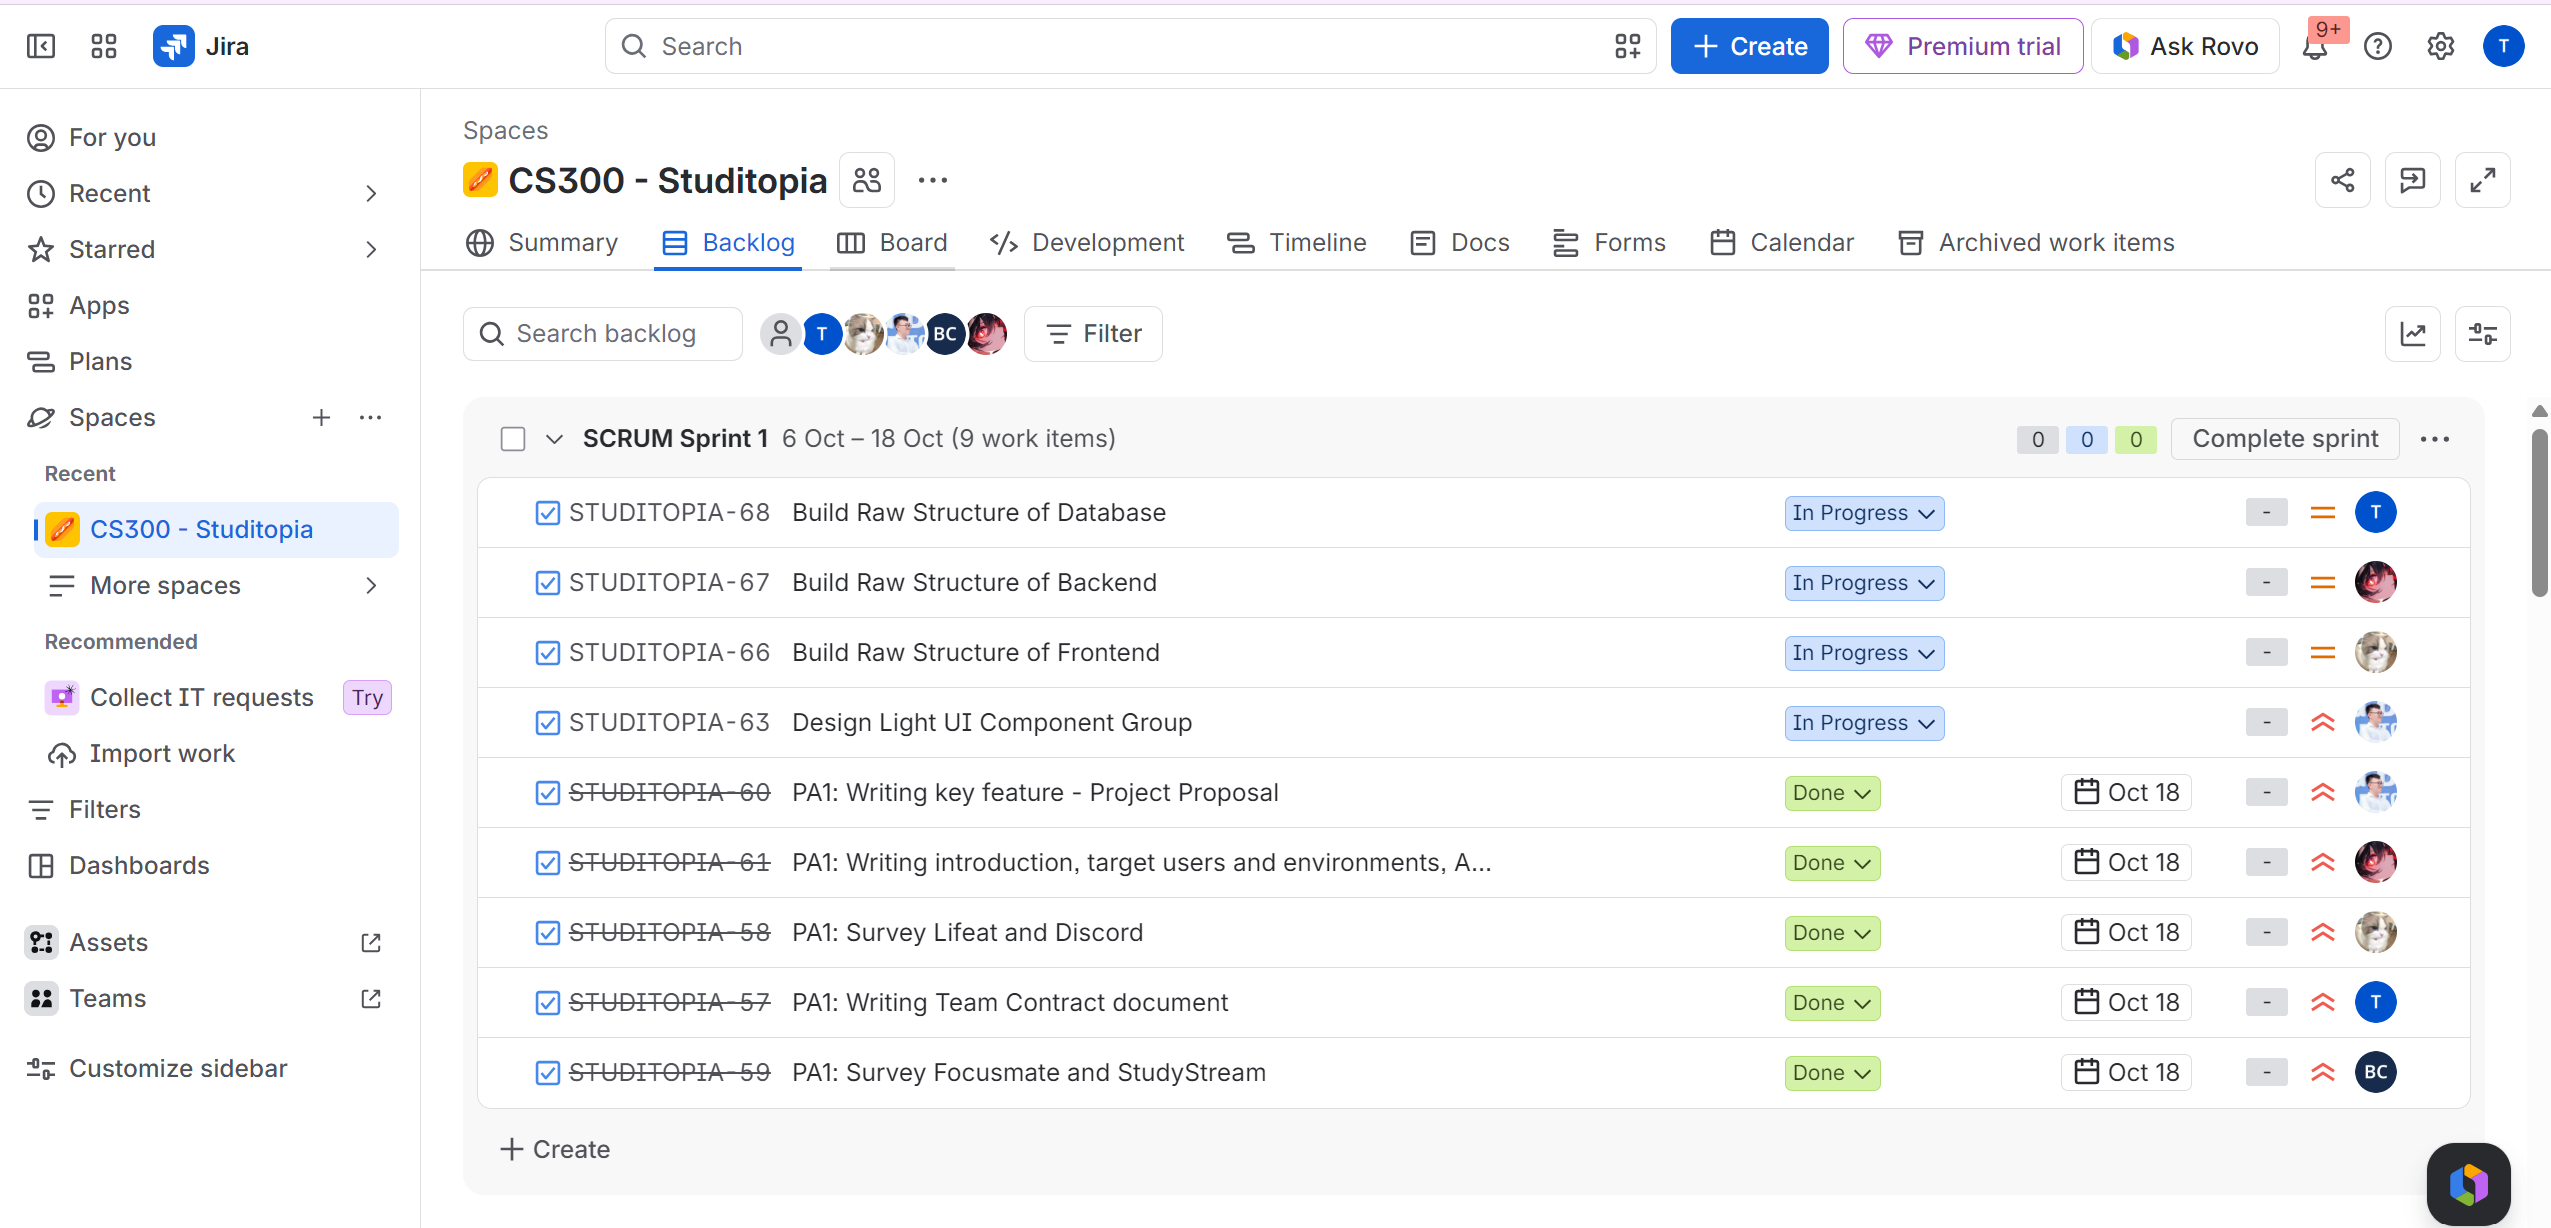
\includegraphics[width=0.8\textwidth]{screenshot/jira-backlog.png}
\end{figure}

\subsubsection{Deadlines and Delays}

\begin{itemize}
    \item Sprint tasks and expected outcomes are agreed during Sprint Planning.
    \item Members report blockers as soon as they are identified.
    \item A member who expects to miss a deadline must notify the team, explain the reason, provide a revised estimate, and help reduce the impact on dependent work.
    \item If necessary, the team reprioritizes or redistributes tasks.
\end{itemize}

\subsection{4. Code, Git, Documentation, and Testing Standards}

\textbf{Performed by:} [Tuan] | \textbf{Reviewed by:} [An] | \textbf{Edited by:} [An]

\subsubsection{Code}

\begin{itemize}
    \item Follow the conventions of the selected language and framework.
    \item Use clear names and keep modules/functions reasonably focused.
    \item Avoid unnecessary duplication.
    \item Keep code readable, maintainable, and testable.
    \item Never commit API keys, passwords, credentials, or other secrets.
\end{itemize}

\subsubsection{Git}

\begin{itemize}
    \item All source code and Markdown documentation are version-controlled.
    \item Use clear commit messages.
    \item Significant changes should be reviewed before merging.
    \item The repository remains private.
\end{itemize}

\begin{figure}[htbp]
    \centering
    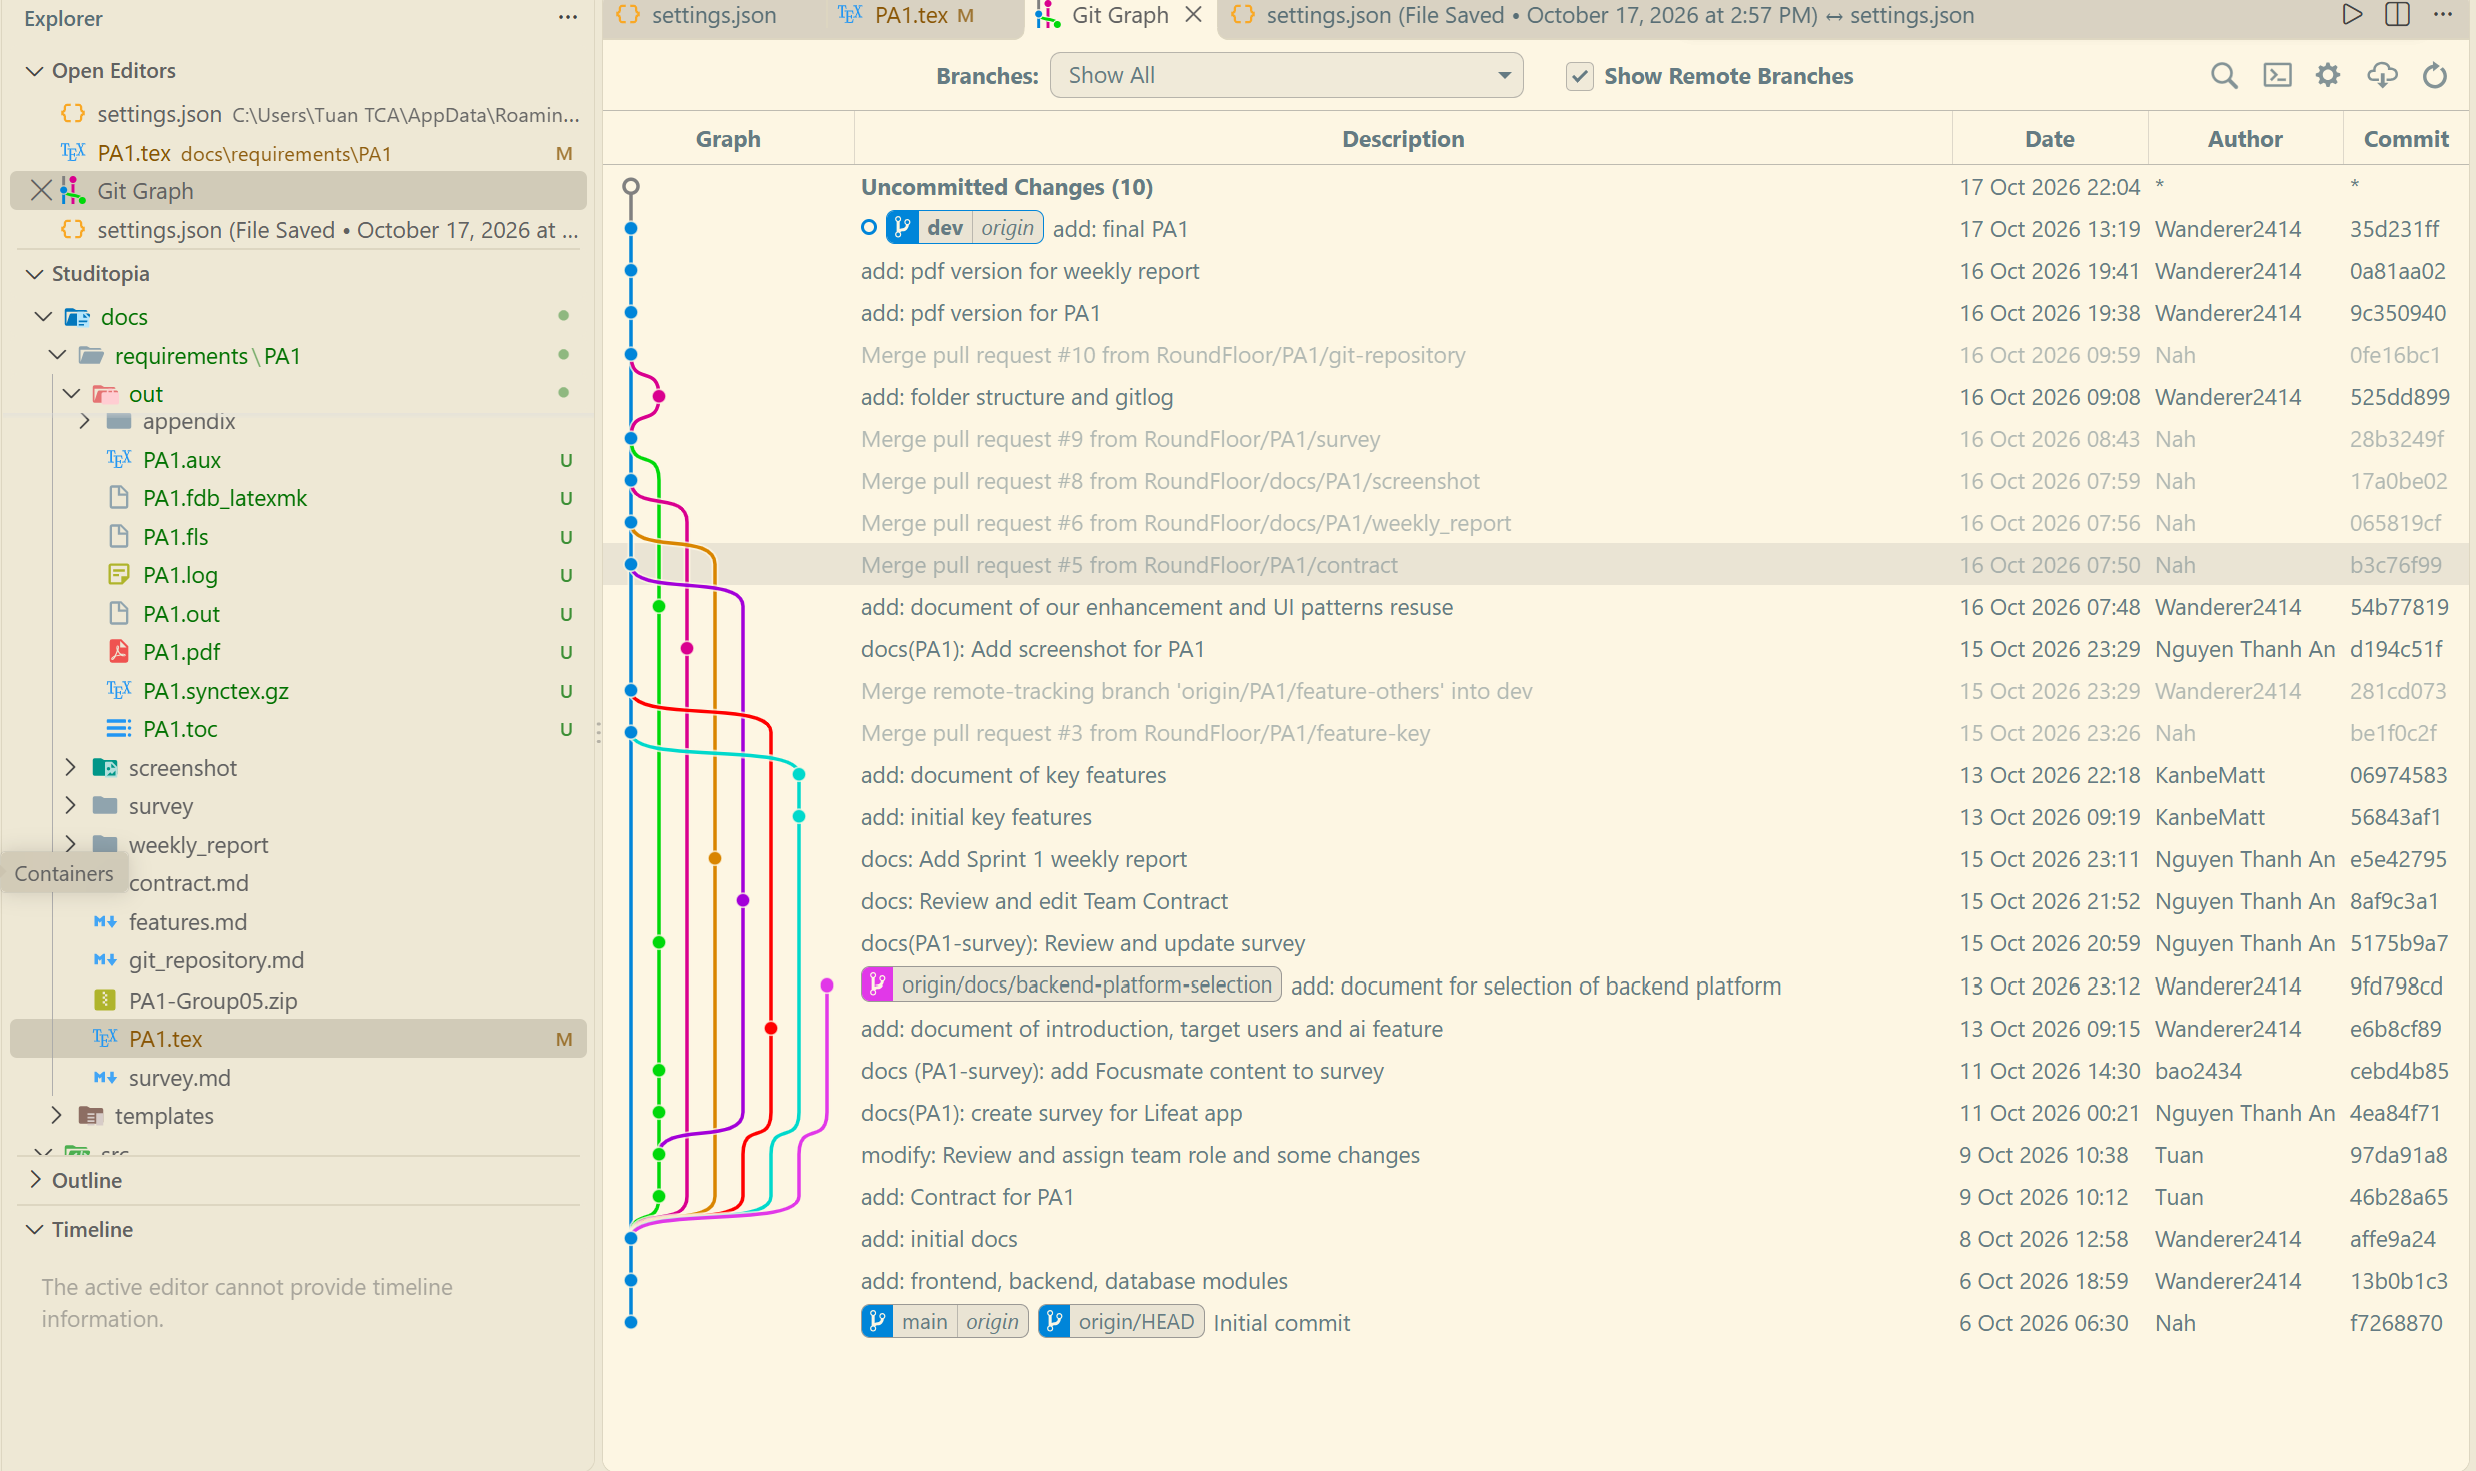
\includegraphics[width=0.8\textwidth]{screenshot/git-graph.png}
\end{figure}

\subsubsection{Documentation}

Documentation is maintained in Markdown and stored in the repository. It includes requirements, analysis/design, testing, management reports, and other required project documents.

Mermaid is used for diagrams whenever practical.

\subsubsection{Testing}

Testing is a shared responsibility. The team performs appropriate component/unit, integration, system, and acceptance testing. A feature is considered complete only after its implementation has been reviewed and appropriately tested.

\subsection{5. Accountability and Performance}

\textbf{Performed by:} [Tuan] | \textbf{Reviewed by:} [An] | \textbf{Edited by:} [An]

Contribution is evaluated using evidence such as:

\begin{itemize}
    \item Completed task-management items
    \item Git commits and pull requests
    \item Code reviews
    \item Testing and documentation
    \item Meeting participation
    \item Communication and timely reporting
    \item Quality and completeness of deliverables
\end{itemize}

Commit count alone is not a measure of contribution.

If a member repeatedly fails to participate or complete assigned work:

\begin{enumerate}
    \item The team discusses the issue with the member.
    \item The cause and corrective action are identified.
    \item Tasks may be adjusted or reassigned to protect project progress.
    \item The issue may be documented with supporting evidence.
    \item Persistent problems may be escalated to the TA or instructor.
\end{enumerate}

\subsection{6. Decision-Making}

\textbf{Performed by:} [Tuan] | \textbf{Reviewed by:} [An] | \textbf{Edited by:} [An]

The team uses the following process:

\begin{enumerate}
    \item \textbf{Discussion:} Seek consensus based on requirements, user value, feasibility, cost, risks, and maintainability.
    \item \textbf{Majority vote:} If consensus cannot be reached, each member has one vote and the majority decides.
    \item \textbf{Escalation:} If a major disagreement remains unresolved, the team consults the TA or instructor.
\end{enumerate}

The primary coordinator facilitates decisions but has no unilateral authority to override the team.

\subsection{7. Conflict Resolution}

\textbf{Performed by:} [Tuan] | \textbf{Reviewed by:} [An] | \textbf{Edited by:} [An]

The team resolves conflicts as follows:

\begin{enumerate}
    \item Clearly identify the issue.
    \item Allow each involved member to explain their position.
    \item Separate facts, requirements, assumptions, and personal preferences.
    \item Discuss possible solutions and consequences.
    \item Reach consensus or use majority vote.
    \item Record decisions that affect the project.
    \item Escalate unresolved issues to the TA or instructor.
\end{enumerate}

Personal attacks, harassment, deliberate exclusion, and withholding important project information are unacceptable.

\subsection{8. AI-Assisted Development}

\textbf{Performed by:} [Tuan] | \textbf{Reviewed by:} [An] | \textbf{Edited by:} [An]

The team may use AI coding tools as development aids in accordance with the requirements and policies officially specified by CS300.

Members must:

\begin{itemize}
    \item Understand AI-assisted code before using it.
    \item Review and test AI-assisted output before integration.
    \item Validate important technical information rather than assuming AI output is correct.
    \item Protect API keys, credentials, private information, and other secrets.
    \item Remain responsible for all submitted code, documentation, and results.
\end{itemize}

AI assistance does not transfer responsibility for the resulting work from the team member to the AI tool.
\begin{figure}[htbp]
    \centering
    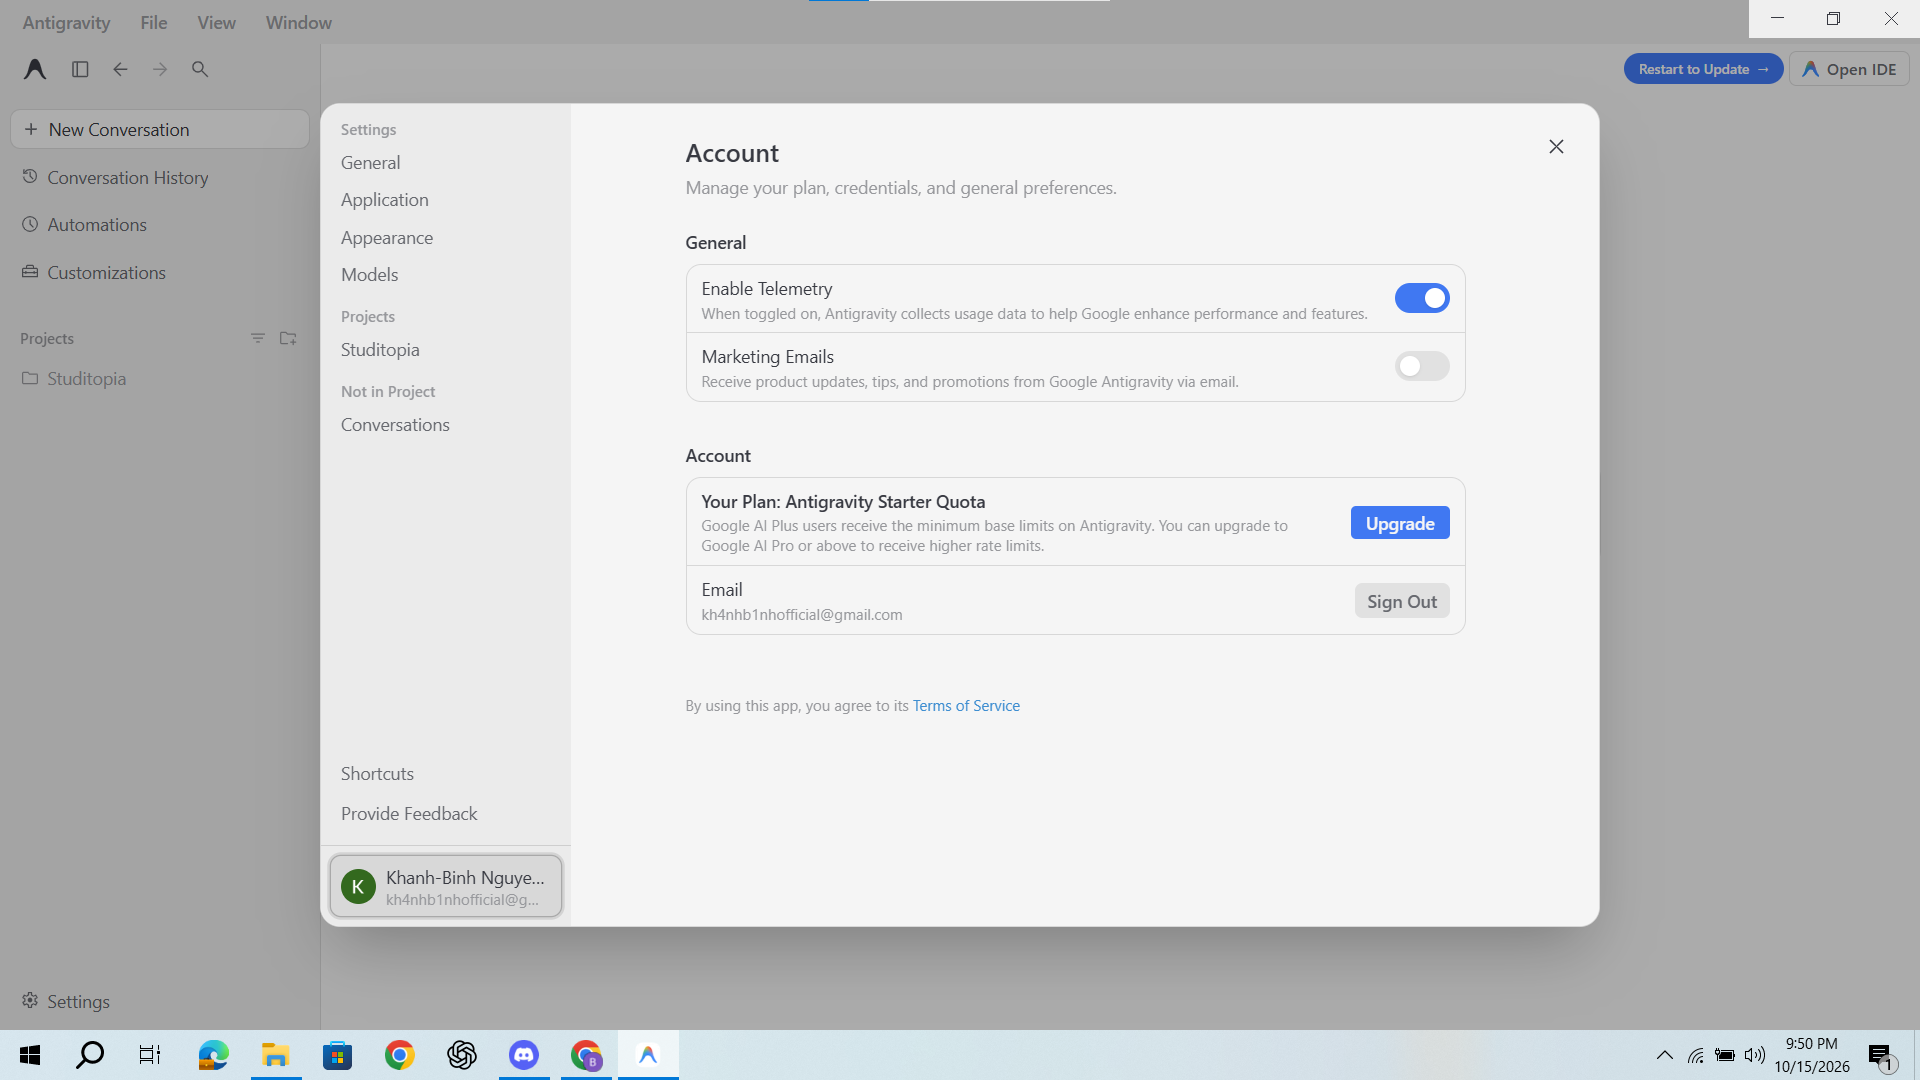
\includegraphics[width=0.8\textwidth]{screenshot/AI_coding_accounts/23125026.png}
\end{figure}

\subsection{9. Change and Risk Management}

\textbf{Performed by:} [Tuan] | \textbf{Reviewed by:} [An] | \textbf{Edited by:} [An]

The team expects requirements and technical decisions to evolve during development.

Before making a significant change, the team considers:

\begin{itemize}
    \item Reason and expected value
    \item Affected requirements and existing work
    \item Effort and dependencies
    \item Technical and project risks
    \item Impact on the current and future Sprint
\end{itemize}

Important changes are discussed before implementation. Risks and blockers are reported early so that the team can reduce rework and protect Sprint goals.

\subsection{10. Contract Review and Updates}

\textbf{Performed by:} [Tuan] | \textbf{Reviewed by:} [An] | \textbf{Edited by:} [An]

The contract is reviewed:

\begin{itemize}
    \item At the beginning of the project.
    \item At the end of each Sprint.
    \item When a significant team-process problem occurs.
    \item When the team agrees that a rule should change.
\end{itemize}

A contract change requires majority approval and must be recorded with its date and revision history. The latest approved version replaces previous versions.

\subsection{12. Team Agreement}

\textbf{Performed by:} [Tuan] | \textbf{Reviewed by:} [An] | \textbf{Edited by:} [An]

By approving this contract, each member agrees to:

\begin{itemize}
    \item Fulfill their assigned responsibilities.
    \item Participate as a full-stack engineer.
    \item Follow the communication and task-management rules.
    \item Report blockers and delays early.
    \item Contribute to development, testing, documentation, and review.
    \item Follow the team's decision-making and conflict-resolution procedures.
    \item Take responsibility for the quality and understanding of their work.
\end{itemize}

\subsubsection{Approval}

\begin{table}[H]
\centering
\begin{tabular}{|c|l|c|c|}
\hline
No. & Full Name & Student ID & Agreement \\
\hline
1 & Nguyễn Thanh An & 24125024 & Agreed \\
\hline
2 & Nguyễn Chí Bảo & 24125025 & Agreed \\
\hline
3 & Trần Nguyễn Khánh Bình & 24125026 & Agreed \\
\hline
4 & Trần Cảnh Anh Tuấn & 24125048 & Agreed \\
\hline
5 & Nguyễn Lê Quốc Huy & 24125100 & Agreed \\
\hline
\end{tabular}
\end{table}

% Appendix
\appendix
% Add \cleardoublepage to move appendices to next page.

\section{Repository structure}
\begin{lstlisting}[
    basicstyle=\ttfamily\footnotesize,
    frame=single,
    breaklines=true,
    columns=fullflexible,
    keepspaces=true
]
.
├── docs
│   ├── analysis-and-design: System analysis, architecture, design diagrams, UML diagrams, and UI/UX design documents.
│   ├── management: Project plans, schedules, task assignments, meeting notes, and progress reports.
│   ├── requirements: Software requirements specifications, user stories, functional requirements, and non-functional requirements.
│   │   ├── PAx: Documentation and deliverables for Project Assignment x
│   │   │   ├── features
│   │   │   ├── screenshot
│   │   │   │   └── AI_coding accounts
│   │   │   ├── survey
│   │   │   │   └── image
│   │   │   │       ├── Focusmate
│   │   │   │       └── Lifeat
│   │   │   └── weekly_report
│   │   │       └── images
│   │   └── proposal
│   └── test
└── src
    ├── backend
    ├── database
    └── frontend
        ├── public
        └── src
            └── assets
\end{lstlisting}
\section{Git log}

\begin{lstlisting}[
    basicstyle=\ttfamily\footnotesize,
    frame=single,
    breaklines=true,
    columns=fullflexible,
    keepspaces=true
]

*   commit 08264a45daa8db8fdefa61dd2e9efa133d2bf9bb
|\  Merge: 28b3249 1fa4069
| | Author: Wanderer2414 <huynguyenlequoc13@gmail.com>
| | Date:   Fri Oct 16 08:52:53 2026 +0700
| | 
| |     WIP on feature/automation-docs: 28b3249 Merge pull request #9 from RoundFloor/PA1/survey
| | 
| * commit 1fa40698b70fe8a5f72b9f7973f66dce436d3397
|/  Author: Wanderer2414 <huynguyenlequoc13@gmail.com>
|   Date:   Fri Oct 16 08:52:53 2026 +0700
|   
|       index on feature/automation-docs: 28b3249 Merge pull request #9 from RoundFloor/PA1/survey
|   
|    .agents/skills/speckit-analyze/SKILL.md          | 259 +++++
|    .agents/skills/speckit-checklist/SKILL.md        | 383 ++++++++
|    .agents/skills/speckit-clarify/SKILL.md          | 291 ++++++
|    .agents/skills/speckit-constitution/SKILL.md     | 179 ++++
|    .agents/skills/speckit-converge/SKILL.md         | 283 ++++++
|    .agents/skills/speckit-implement/SKILL.md        | 226 +++++
|    .agents/skills/speckit-plan/SKILL.md             | 166 ++++
|    .agents/skills/speckit-specify/SKILL.md          | 345 +++++++
|    .agents/skills/speckit-tasks/SKILL.md            | 215 +++++
|    .agents/skills/speckit-taskstoissues/SKILL.md    | 117 +++
|    .specify/.gitignore                              |  14 +
|    .specify/init-options.json                       |  10 +
|    .specify/integration.json                        |  15 +
|    .specify/integrations/agy.manifest.json          |  17 +
|    .specify/integrations/speckit.manifest.json      |  19 +
|    .specify/memory/.constitution-template.json      |   4 +
|    .specify/memory/constitution.md                  |  50 +
|    .specify/scripts/bash/check-prerequisites.sh     | 243 +++++
|    .specify/scripts/bash/common.sh                  | 942 +++++++++++++++++++
|    .specify/scripts/bash/create-new-feature.sh      | 504 ++++++++++
|    .specify/scripts/bash/resolve-template.sh        |  57 ++
|    .specify/scripts/bash/setup-plan.sh              |  85 ++
|    .specify/scripts/bash/setup-tasks.sh             |  94 ++
|    .specify/templates/checklist-template.md         |  45 +
|    .specify/templates/constitution-template.md      |  50 +
|    .specify/templates/plan-template.md              | 113 +++
|    .specify/templates/spec-template.md              | 131 +++
|    .specify/templates/tasks-template.md             | 252 +++++
|    .specify/workflows/speckit/workflow.yml          |  74 ++
|    .specify/workflows/workflow-registry.json        |  13 +
|    node_modules/.bin/opencode                       |   1 +
|    node_modules/.package-lock.json                  |  64 ++
|    node_modules/opencode-ai/LICENSE                 |  21 +
|    node_modules/opencode-ai/bin/opencode.exe        | Bin 0 -> 185993344 bytes
|    node_modules/opencode-ai/package.json            |  34 +
|    node_modules/opencode-ai/postinstall.mjs         | 189 ++++
|    .../opencode-linux-x64-baseline/bin/opencode     | Bin 0 -> 185993344 bytes
|    .../opencode-linux-x64-baseline/package.json     |  11 +
|    node_modules/opencode-linux-x64/bin/opencode     | Bin 0 -> 185993344 bytes
|    node_modules/opencode-linux-x64/package.json     |  11 +
|    40 files changed, 5527 insertions(+)
|   
*   commit 28b3249f271b9ca8a7d0bea41cd0b6ada1e6c338
|\  Merge: 17a0be0 54b7781
| | Author: Nah <huynguyenlequoc13@gmail.com>
| | Date:   Fri Oct 16 08:43:19 2026 +0700
| | 
| |     Merge pull request #9 from RoundFloor/PA1/survey
| |     
| |     Pa1/survey
| | 
| * commit 54b7781989b8028759038b4e446c28c7aeb692f4
| | Author: Wanderer2414 <huynguyenlequoc13@gmail.com>
| | Date:   Fri Oct 16 07:48:21 2026 +0700
| | 
| |     add: document of our enhancement and UI patterns resuse
| | 
| |  docs/requirements/PA1/survey.md        | 312 +++++++++++++++++++++++++++++
| |  docs/requirements/PA1/survey/survey.md |  49 +++++
| |  2 files changed, 361 insertions(+)
| | 
| * commit 5175b9a7d62175db0e9aea579a69b47cbcff3149
| | Author: Nguyen Thanh An <ntan2419@apcs.fitus.edu.vn>
| | Date:   Thu Oct 15 20:59:30 2026 +0700
| | 
| |     docs(PA1-survey): Review and update survey
| | 
| |  docs/requirements/PA1/survey/survey.md | 88 +++++++++++++++++-------------
| |  1 file changed, 51 insertions(+), 37 deletions(-)
| | 
| * commit cebd4b8577513d3873a987eb679ed7328997cb23
| | Author: bao2434 <ncbao2434@apcs.fitus.edu.vn>
| | Date:   Sun Oct 11 14:30:48 2026 +0700
| | 
| |     docs (PA1-survey): add Focusmate content to survey
| | 
| |  .../PA1/survey/image/Focusmate/book_session.png  | Bin 0 -> 117090 bytes
| |  .../PA1/survey/image/Focusmate/calendar.png      | Bin 0 -> 292086 bytes
| |  .../PA1/survey/image/Focusmate/join_session.png  | Bin 0 -> 43112 bytes
| |  .../survey/image/Focusmate/pre_session_setup.png | Bin 0 -> 88149 bytes
| |  .../PA1/survey/image/Focusmate/session.png       | Bin 0 -> 75615 bytes
| |  docs/requirements/PA1/survey/survey.md           |  44 ++++++++++++++++++-
| |  6 files changed, 42 insertions(+), 2 deletions(-)
| | 
| * commit 4ea84f71dfce3eb2f2877bb44d3de1db1361bc70
| | Author: Nguyen Thanh An <ntan2419@apcs.fitus.edu.vn>
| | Date:   Sun Oct 11 00:21:22 2026 +0700
| | 
| |     docs(PA1): create survey for Lifeat app
| | 
| |  .../PA1/survey/image/Lifeat/calendar_button.png  | Bin 0 -> 2045 bytes
| |  .../PA1/survey/image/Lifeat/chat.png             | Bin 0 -> 55130 bytes
| |  .../survey/image/Lifeat/explore_mode_screen.png  | Bin 0 -> 1024798 bytes
| |  .../survey/image/Lifeat/focus_mode_screen.png    | Bin 0 -> 2685300 bytes
| |  .../PA1/survey/image/Lifeat/invite_button.png    | Bin 0 -> 3264 bytes
| |  .../PA1/survey/image/Lifeat/invite_friend.png    | Bin 0 -> 12648 bytes
| |  .../PA1/survey/image/Lifeat/media_button.png     | Bin 0 -> 1637 bytes
| |  .../PA1/survey/image/Lifeat/media_video.png      | Bin 0 -> 119130 bytes
| |  .../PA1/survey/image/Lifeat/media_window.png     | Bin 0 -> 28615 bytes
| |  .../PA1/survey/image/Lifeat/notes_button.png     | Bin 0 -> 1709 bytes
| |  .../PA1/survey/image/Lifeat/notes_create.png     | Bin 0 -> 10751 bytes
| |  .../PA1/survey/image/Lifeat/notes_window.png     | Bin 0 -> 8948 bytes
| |  .../PA1/survey/image/Lifeat/plan_mode_screen.png | Bin 0 -> 23608 bytes
| |  .../PA1/survey/image/Lifeat/plan_project.png     | Bin 0 -> 17901 bytes
| |  .../PA1/survey/image/Lifeat/project_create.png   | Bin 0 -> 21159 bytes
| |  .../PA1/survey/image/Lifeat/project_edit.png     | Bin 0 -> 10461 bytes
| |  .../PA1/survey/image/Lifeat/project_manager.png  | Bin 0 -> 21115 bytes
| |  .../PA1/survey/image/Lifeat/sound_button.png     | Bin 0 -> 1822 bytes
| |  .../PA1/survey/image/Lifeat/sound_window.png     | Bin 0 -> 39190 bytes
| |  .../PA1/survey/image/Lifeat/space_button.png     | Bin 0 -> 2361 bytes
| |  .../PA1/survey/image/Lifeat/space_favorite.png   | Bin 0 -> 355928 bytes
| |  .../survey/image/Lifeat/space_favorite_list.png  | Bin 0 -> 18982 bytes
| |  .../PA1/survey/image/Lifeat/space_search.png     | Bin 0 -> 413398 bytes
| |  .../PA1/survey/image/Lifeat/space_window.png     | Bin 0 -> 372873 bytes
| |  .../PA1/survey/image/Lifeat/task_button.png      | Bin 0 -> 1384 bytes
| |  .../PA1/survey/image/Lifeat/task_create.png      | Bin 0 -> 9233 bytes
| |  .../PA1/survey/image/Lifeat/task_edit.png        | Bin 0 -> 12507 bytes
| |  .../PA1/survey/image/Lifeat/task_info1.png       | Bin 0 -> 16981 bytes
| |  .../PA1/survey/image/Lifeat/task_info2.png       | Bin 0 -> 17532 bytes
| |  .../PA1/survey/image/Lifeat/task_schedule.png    | Bin 0 -> 11137 bytes
| |  .../PA1/survey/image/Lifeat/task_window.png      | Bin 0 -> 7607 bytes
| |  .../PA1/survey/image/Lifeat/timer_button.png     | Bin 0 -> 1706 bytes
| |  .../PA1/survey/image/Lifeat/timer_group.png      | Bin 0 -> 10418 bytes
| |  .../PA1/survey/image/Lifeat/timer_personal.png   | Bin 0 -> 10241 bytes
| |  .../PA1/survey/image/Lifeat/timer_task.png       | Bin 0 -> 8268 bytes
| |  .../PA1/survey/image/Lifeat/timer_task_play.png  | Bin 0 -> 65360 bytes
| |  .../PA1/survey/image/Lifeat/video_call.png       | Bin 0 -> 193776 bytes
| |  docs/requirements/PA1/survey/survey.md           | 226 +++++++++++++++++++
| |  38 files changed, 226 insertions(+)
| |   
* |   commit 17a0be02a9257bfabaa5e9b43464e55f338fe98b
|\ \  Merge: 065819c d194c51
| | | Author: Nah <huynguyenlequoc13@gmail.com>
| | | Date:   Fri Oct 16 07:59:34 2026 +0700
| | | 
| | |     Merge pull request #8 from RoundFloor/docs/PA1/screenshot
| | |     
| | |     docs(PA1): Add screenshot for PA1
| | | 
| * | commit d194c51f4acefa70b9defe3ec803c60f914a179a
| | | Author: Nguyen Thanh An <ntan2419@apcs.fitus.edu.vn>
| | | Date:   Thu Oct 15 23:29:21 2026 +0700
| | | 
| | |     docs(PA1): Add screenshot for PA1
| | | 
| | |  .../screenshot/AI_coding accounts/23125026.png   | Bin 0 -> 169067 bytes
| | |  .../screenshot/AI_coding accounts/24125025.png   | Bin 0 -> 272385 bytes
| | |  .../screenshot/AI_coding accounts/24125048.png   | Bin 0 -> 122823 bytes
| | |  .../screenshot/AI_coding accounts/24125100.png   | Bin 0 -> 104635 bytes
| | |  .../PA1/screenshot/jira_screenshot.jpeg          | Bin 0 -> 73736 bytes
| | |  5 files changed, 0 insertions(+), 0 deletions(-)
| | |   
* | |   commit 065819cf69a690c8c5f99f56f6959c75c653ed5d
|\ \ \  Merge: b3c76f9 e5e4279
| | | | Author: Nah <huynguyenlequoc13@gmail.com>
| | | | Date:   Fri Oct 16 07:56:33 2026 +0700
| | | | 
| | | |     Merge pull request #6 from RoundFloor/docs/PA1/weekly_report
| | | |     
| | | |     docs: Add Sprint 1 weekly report
| | | | 
| * | | commit e5e42795a20c6e9dfffb3ba8887a1236bf9128ca
| |/ /  Author: Nguyen Thanh An <ntan2419@apcs.fitus.edu.vn>
| | |   Date:   Thu Oct 15 23:11:09 2026 +0700
| | |   
| | |       docs: Add Sprint 1 weekly report
| | |   
| | |    .../weekly_report/images/week1_jira_task.jpeg | Bin 0 -> 97267 bytes
| | |    .../weekly_report/images/week2_jira_task.jpeg | Bin 0 -> 117716 bytes
| | |    .../PA1/weekly_report/weekly_report1.md       | 107 ++++++++++++++++
| | |    .../PA1/weekly_report/weekly_report2.md       | 116 ++++++++++++++++++
| | |    4 files changed, 223 insertions(+)
| | |   
* | |   commit b3c76f99327c9863119a8656c36f8f04a255061b
|\ \ \  Merge: 281cd07 8af9c3a
| | | | Author: Nah <huynguyenlequoc13@gmail.com>
| | | | Date:   Fri Oct 16 07:50:01 2026 +0700
| | | | 
| | | |     Merge pull request #5 from RoundFloor/PA1/contract
| | | |     
| | | |     Pa1/contract
| | | | 
| * | | commit 8af9c3a1c4441e6488c5504363bd6d4d791c0b33
| | |/  Author: Nguyen Thanh An <ntan2419@apcs.fitus.edu.vn>
| |/|   Date:   Thu Oct 15 21:52:00 2026 +0700
| | |   
| | |       docs: Review and edit Team Contract
| | |   
| | |    docs/requirements/PA1/contract.md | 80 ++++++++++---------------------
| | |    1 file changed, 26 insertions(+), 54 deletions(-)
| | | 
| * | commit 97da91a8def3f41e9cbe80756ca68a4a492a738a
| | | Author: Tuan <tuan06nbk@gmail.com>
| | | Date:   Fri Oct 9 10:38:45 2026 +0700
| | | 
| | |     modify: Review and assign team role and some changes
| | | 
| | |  docs/requirements/PA1/contract.md | 13 +++++++------
| | |  1 file changed, 7 insertions(+), 6 deletions(-)
| | | 
| * | commit 46b28a651fb835aae3f4ad7bb10f40885484d126
| |/  Author: Tuan <tuan06nbk@gmail.com>
| |   Date:   Fri Oct 9 10:12:31 2026 +0700
| |   
| |       add: Contract for PA1
| |   
| |    docs/requirements/PA1/contract.md | 259 ++++++++++++++++++++++++++++++++
| |    1 file changed, 259 insertions(+)
| |   
* |   commit 281cd07341a07ab262b74d987b85abbefa36f1bf
|\ \  Merge: be1f0c2 e6b8cf8
| | | Author: Wanderer2414 <huynguyenlequoc13@gmail.com>
| | | Date:   Thu Oct 15 23:29:07 2026 +0700
| | | 
| | |     Merge remote-tracking branch 'origin/PA1/feature-others' into dev
| | | 
| * | commit e6b8cf895a7f1bf75003ab68919d63bbb04af057
| |/  Author: Wanderer2414 <huynguyenlequoc13@gmail.com>
| |   Date:   Tue Oct 13 09:15:08 2026 +0700
| |   
| |       add: document of introduction, target users and ai feature
| |   
| |    docs/requirements/PA1/features.md               | 31 +++++++++++++++++++
| |    docs/requirements/PA1/features/0-title.md       |  1 +
| |    .../requirements/PA1/features/1-introduction.md | 10 ++++++
| |    .../PA1/features/3-targetuser-platform.md       |  9 ++++++
| |    docs/requirements/PA1/features/5-ai-feature.md  | 10 ++++++
| |    5 files changed, 61 insertions(+)
| |   
* |   commit be1f0c2f7e63a3cf02f879f9856cc32e2bc2517e
|\ \  Merge: affe9a2 0697458
| |/  Author: Nah <huynguyenlequoc13@gmail.com>
|/|   Date:   Thu Oct 15 23:26:33 2026 +0700
| |   
| |       Merge pull request #3 from RoundFloor/PA1/feature-key
| |       
| |       Pa1/feature key
| | 
| * commit 06974583dd621e8d0c482905b1f732c5d3f7c974
| | Author: KanbeMatt <khanhbinh08062006@gmail.com>
| | Date:   Tue Oct 13 22:18:36 2026 +0700
| | 
| |     add: document of key features
| | 
| |  docs/requirements/PA1/features.md                |  1 +
| |  docs/requirements/PA1/features/4-key-features.md | 31 ++++++++++++++++++++
| |  2 files changed, 32 insertions(+)
| | 
| * commit 56843af1899e7c27479e3ce88eb89120aeb7b49b
|/  Author: KanbeMatt <khanhbinh08062006@gmail.com>
|   Date:   Tue Oct 13 09:19:31 2026 +0700
|   
|       add: initial key features
|   
|    docs/requirements/PA1/features/4-key-features.md | 0
|    1 file changed, 0 insertions(+), 0 deletions(-)
|   
| * commit 9fd798cdb0f5360ef300b527c333f68deb943ab0
|/  Author: Wanderer2414 <huynguyenlequoc13@gmail.com>
|   Date:   Tue Oct 13 23:12:59 2026 +0700
|   
|       add: document for selection of backend platform
|   
|    docs/requirements/backend-platform-selection.md  | 937 +++++++++++++++++++
|    .../1-backend-platform-selection.md              | 461 +++++++++
|    .../2-backend-comparision.md                     | 477 ++++++++++
|    3 files changed, 1875 insertions(+)
| 
* commit affe9a2472dad57b8974aeb4c45b2b288ebf4d9b
| Author: Wanderer2414 <nlqhuy2414@apcs.fitus.edu.vn>
| Date:   Thu Oct 8 12:58:27 2026 +0700
| 
|     add: initial docs
| 
|  .vscode/tasks.json                                | 22 +++++++++++++++++++++
|  docs/requirements/proposal.md                     |  4 ++++
|  docs/requirements/proposal/1-overview.md          |  0
|  docs/requirements/proposal/2-userstory.md         |  0
|  .../proposal/3-functional-requirement.md          |  0
|  .../proposal/4-nonfunctional-requirement.md       |  0
|  6 files changed, 26 insertions(+)
| 
* commit 13b0b1c3e96246d7e65bcf0e23f0dadd889120ba
| Author: Wanderer2414 <nlqhuy2414@apcs.fitus.edu.vn>
| Date:   Tue Oct 6 18:59:53 2026 +0700
| 
|     add: frontend, backend, database modules
| 
|  .gitmodules  | 12 ++++++++++++
|  src/backend  |  1 +
|  src/database |  1 +
|  src/frontend |  1 +
|  4 files changed, 15 insertions(+)
| 
* commit f7268870c512fb057fdbd20ea5aa29217cdab064
  Author: Nah <huynguyenlequoc13@gmail.com>
  Date:   Tue Oct 6 06:30:07 2026 +0700
  
      Initial commit
  
   LICENSE | 373 ++++++++++++++++++++++++++++++++++++++++++++++++++++++++++++++
   1 file changed, 373 insertions(+)
\end{lstlisting}

\section{Jira usage proof}

\begin{figure}[htbp]
    \centering
    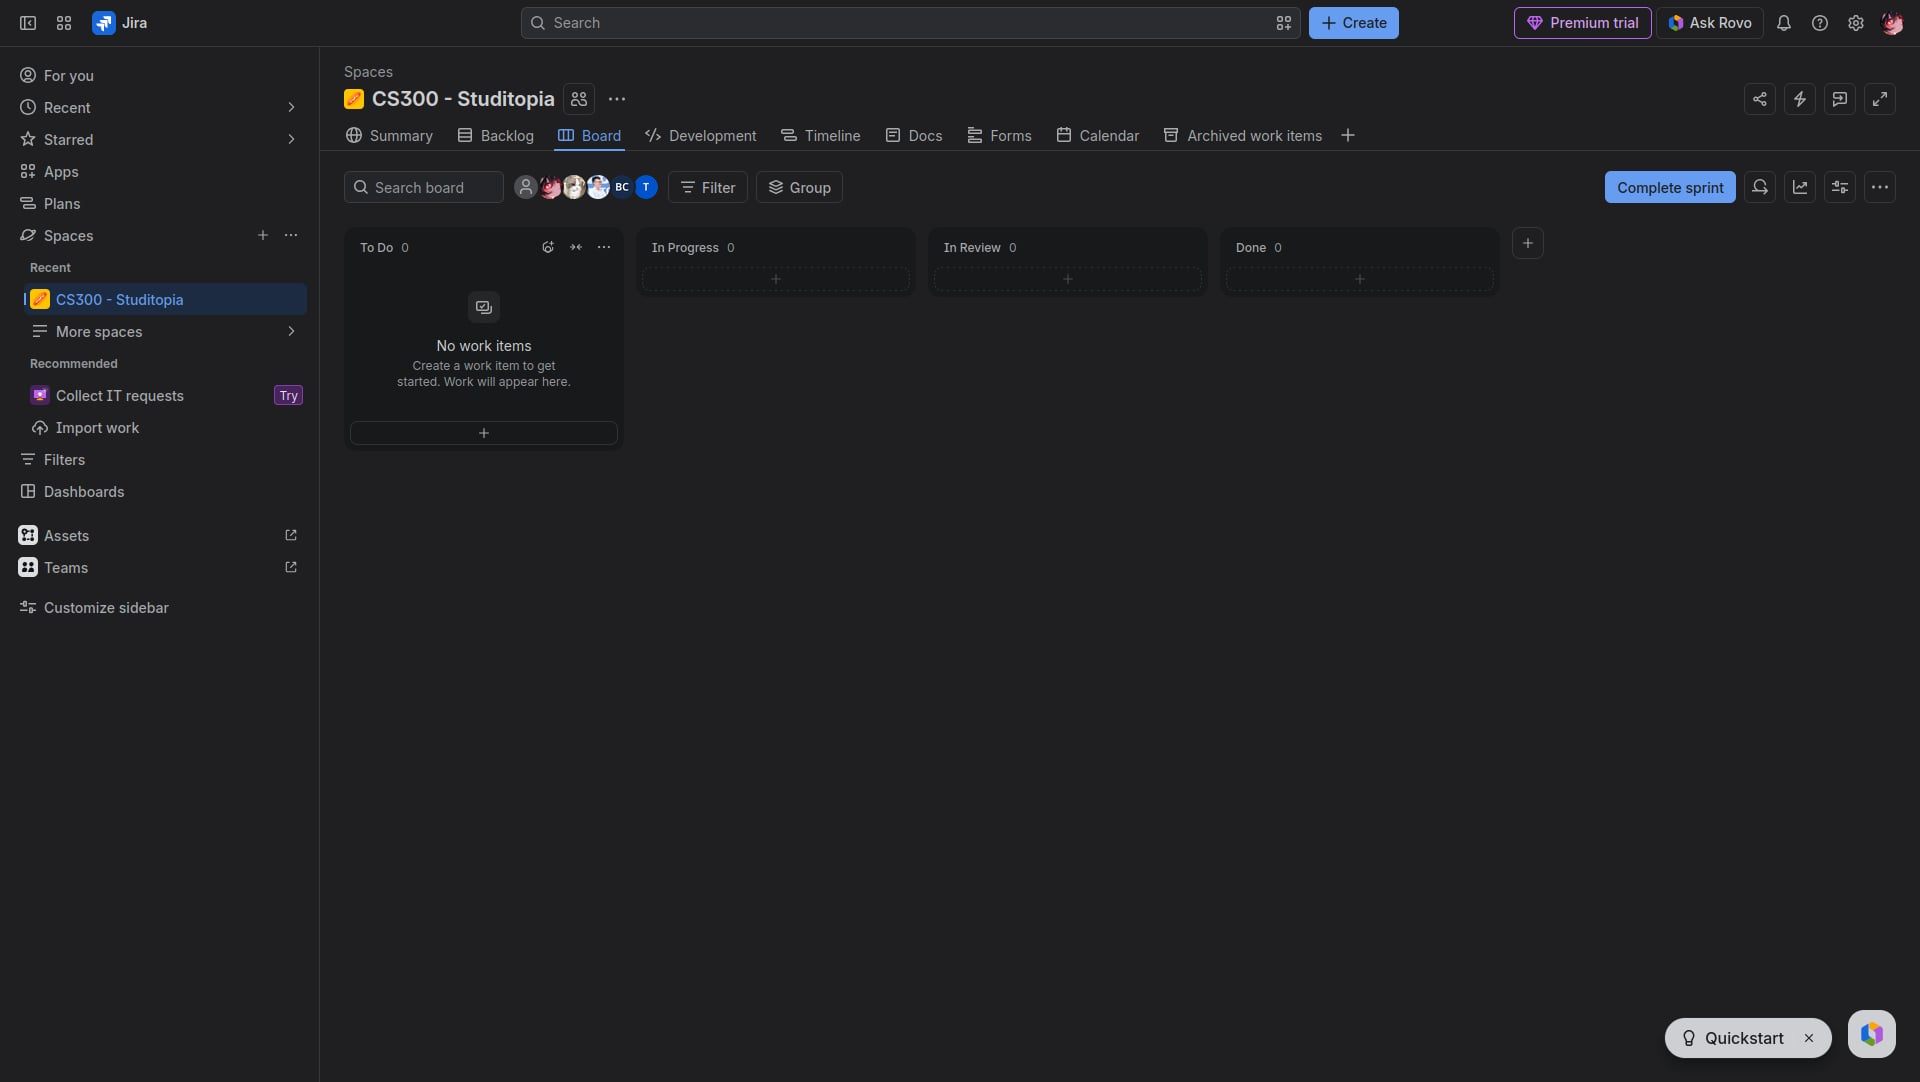
\includegraphics[width=0.8\textwidth]{screenshot/jira_screenshot.jpeg}
\end{figure}

\section{AI coding accounts proof}

\begin{figure}[htbp]
    \centering

    % Row 1
    \begin{subfigure}{0.3\textwidth}
        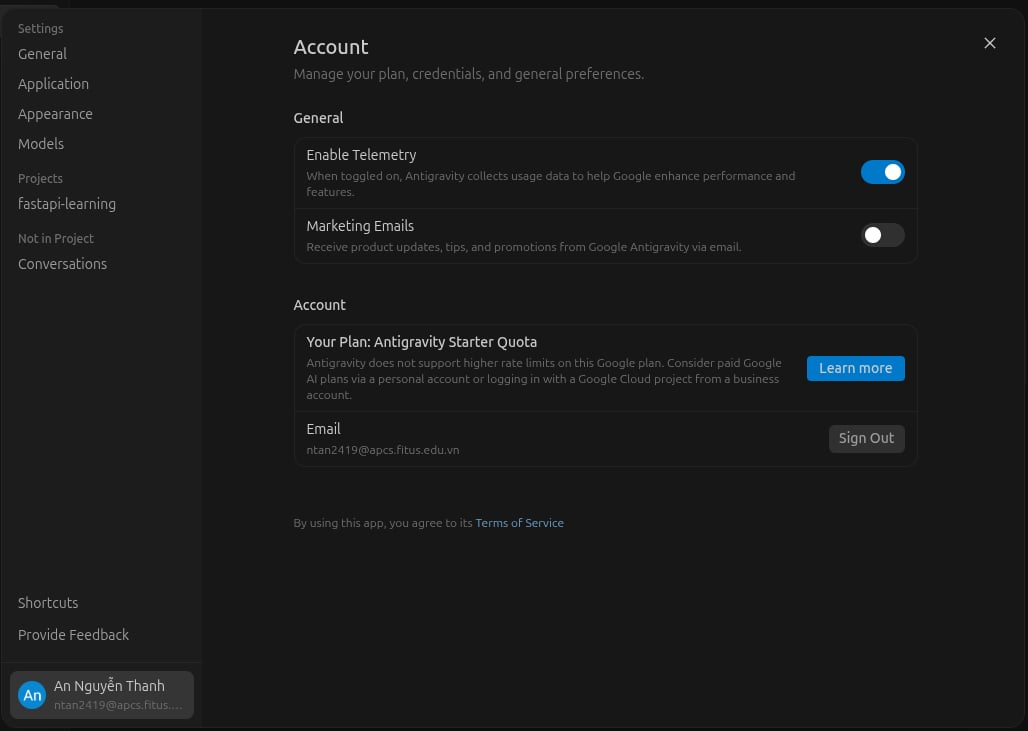
\includegraphics[width=\linewidth]{screenshot/AI_coding_accounts/24125024.png}
        \caption{24125024}
    \end{subfigure}
    \hfill
    \begin{subfigure}{0.3\textwidth}
        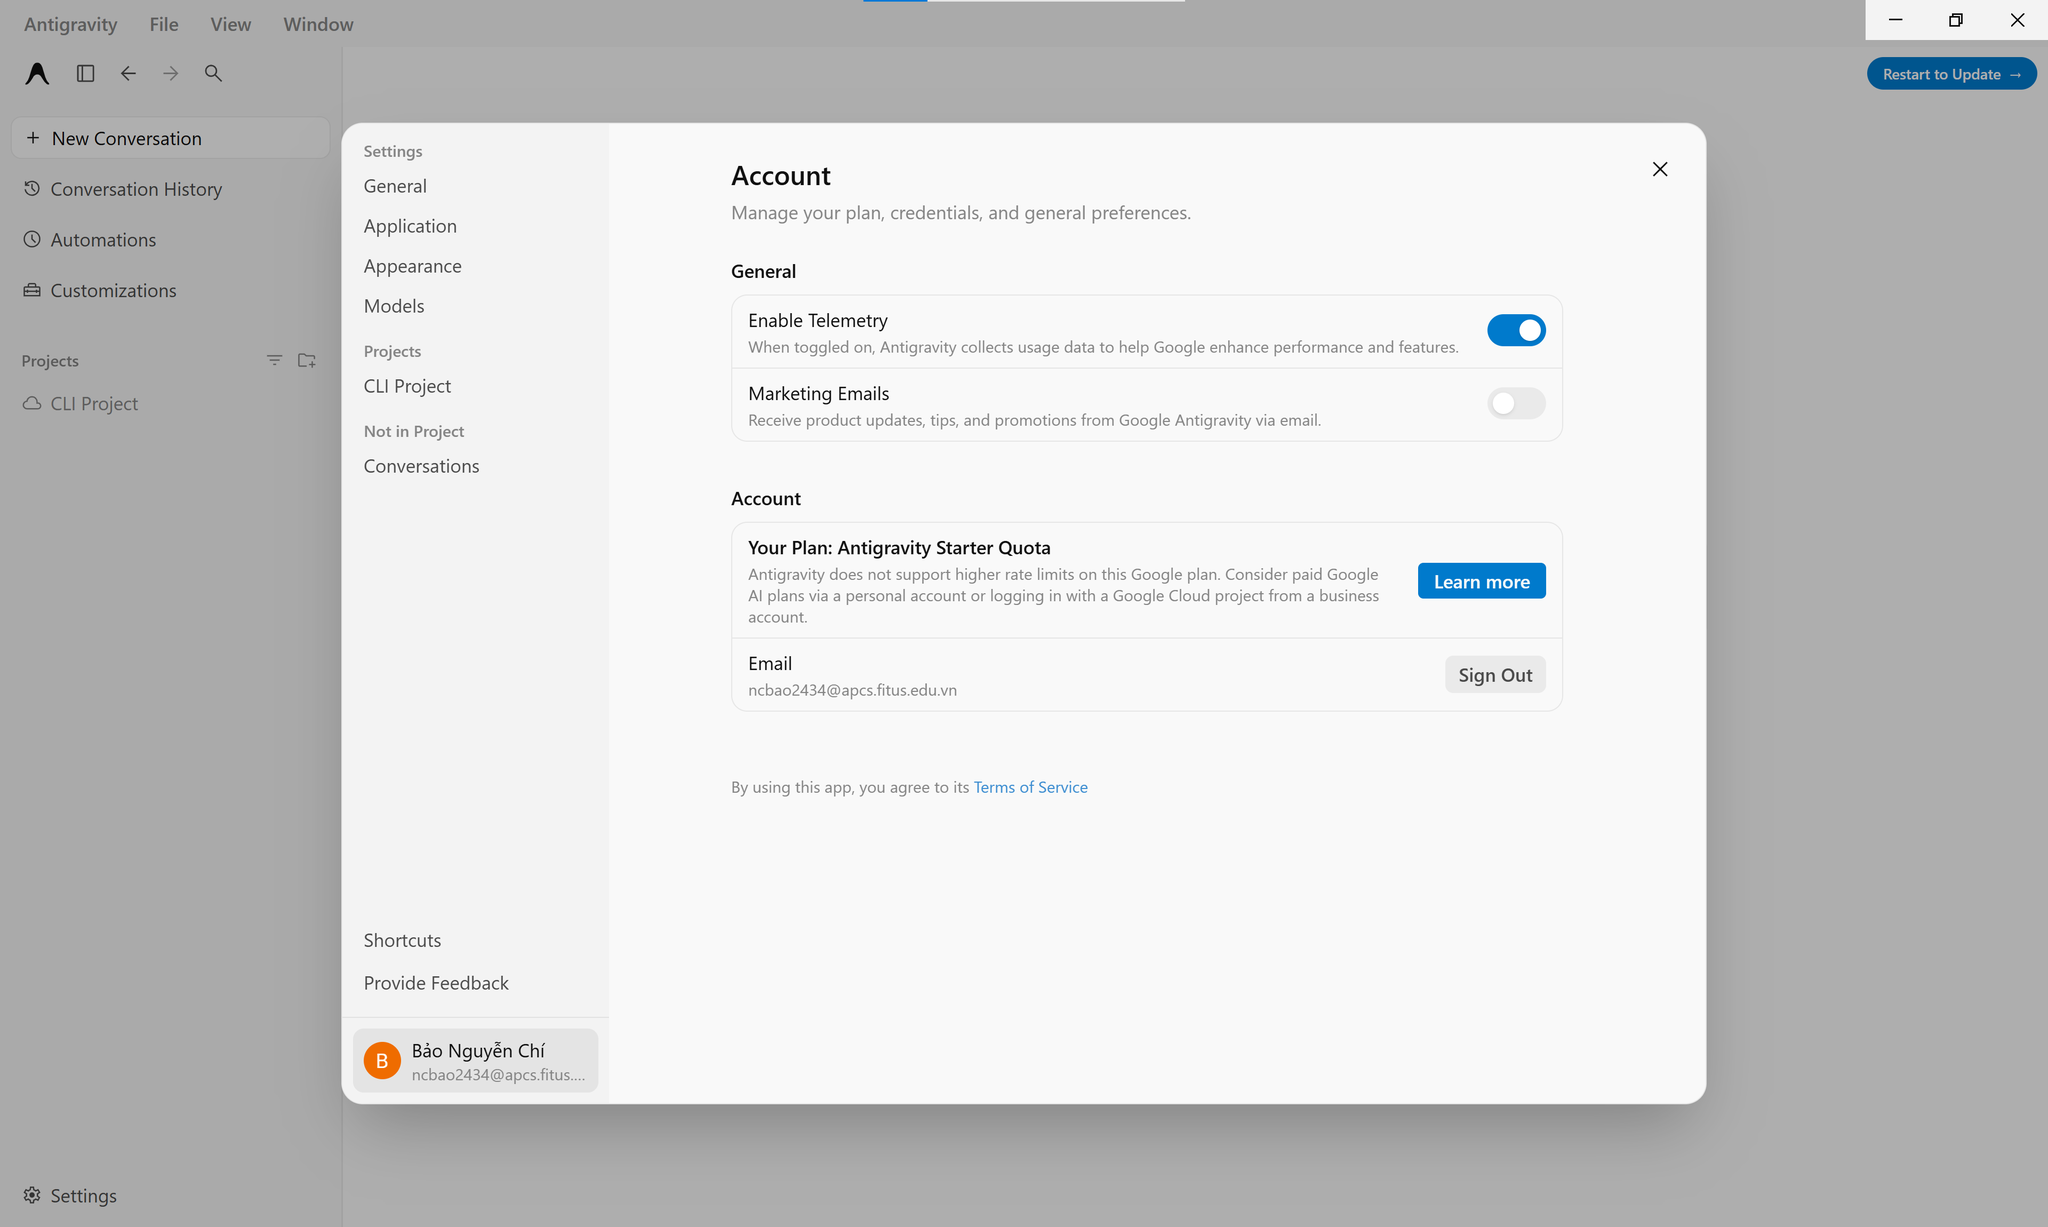
\includegraphics[width=\linewidth]{screenshot/AI_coding_accounts/24125025.png}
        \caption{24125025}
    \end{subfigure}
    \hfill
    \begin{subfigure}{0.3\textwidth}
        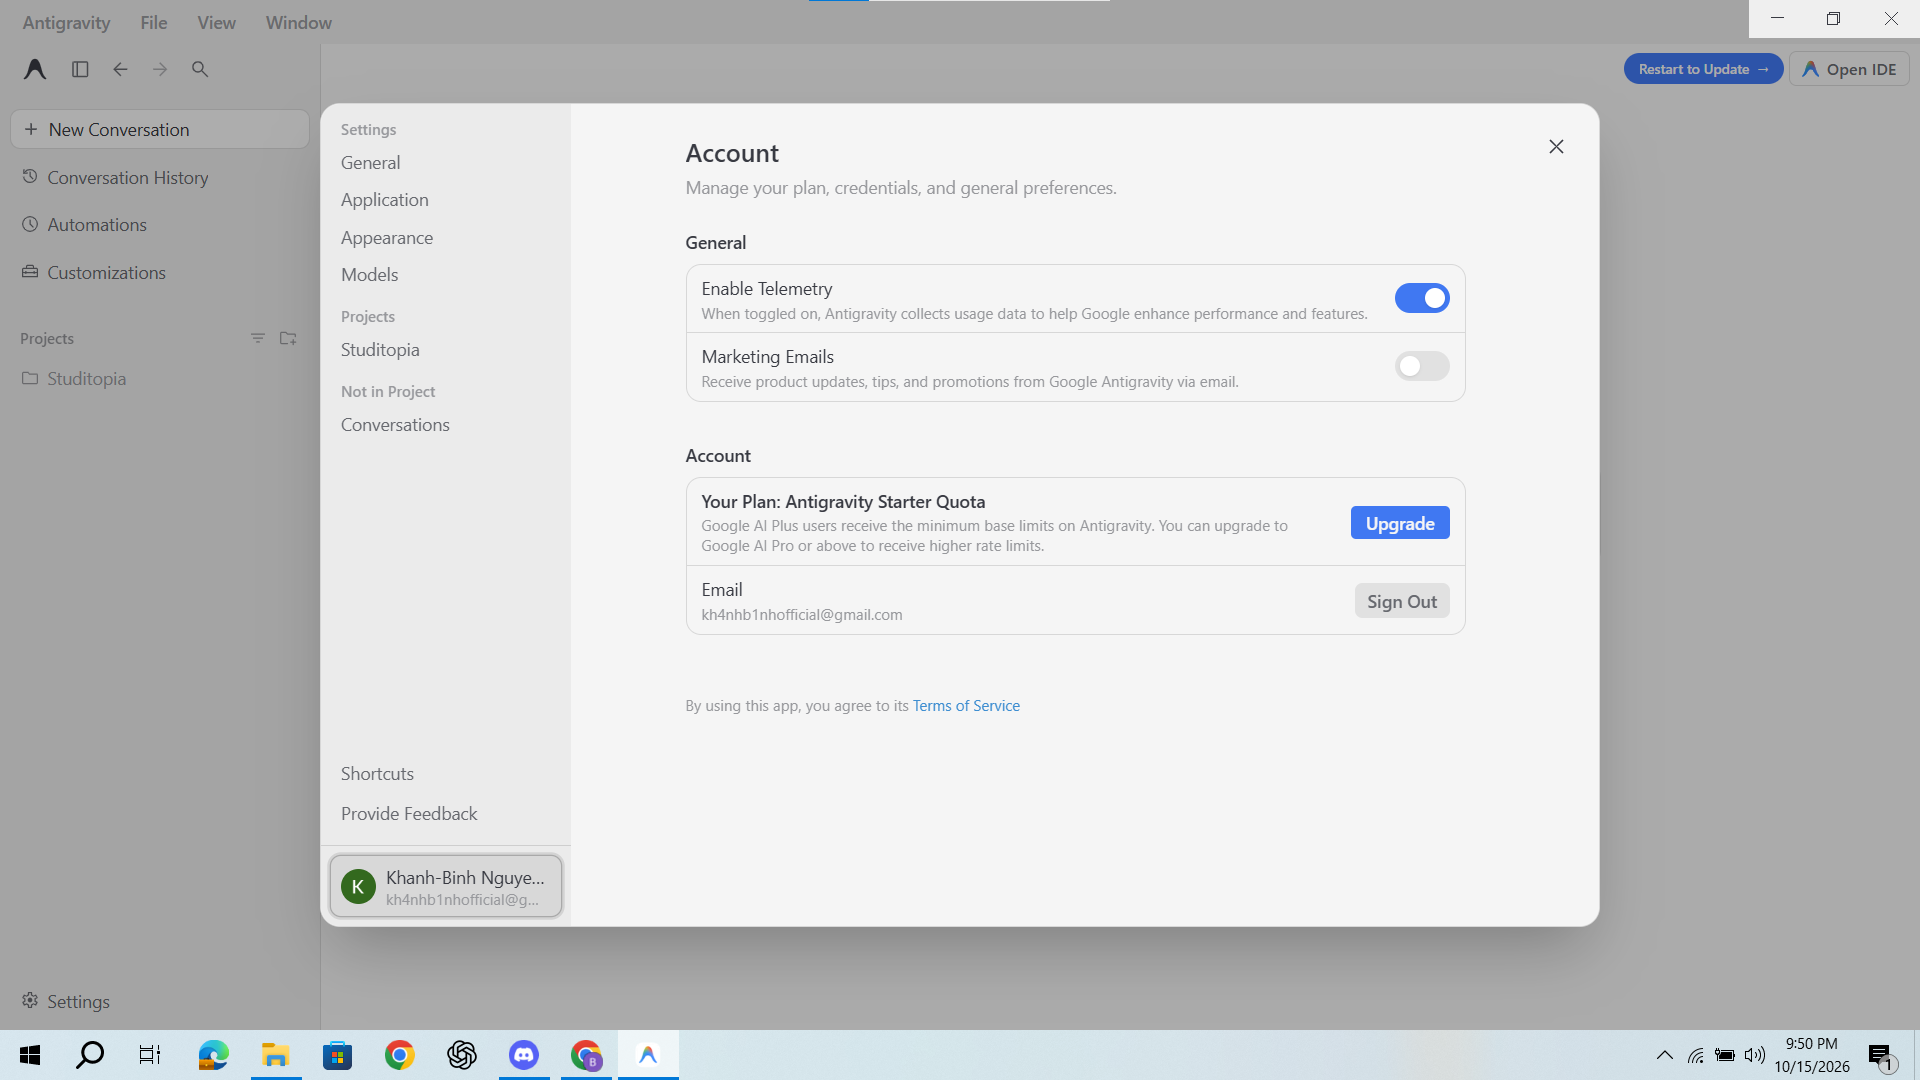
\includegraphics[width=\linewidth]{screenshot/AI_coding_accounts/24125026.png}
        \caption{24125026}
    \end{subfigure}

    \vspace{0.5em}

    % Row 2
    \begin{subfigure}{0.3\textwidth}
        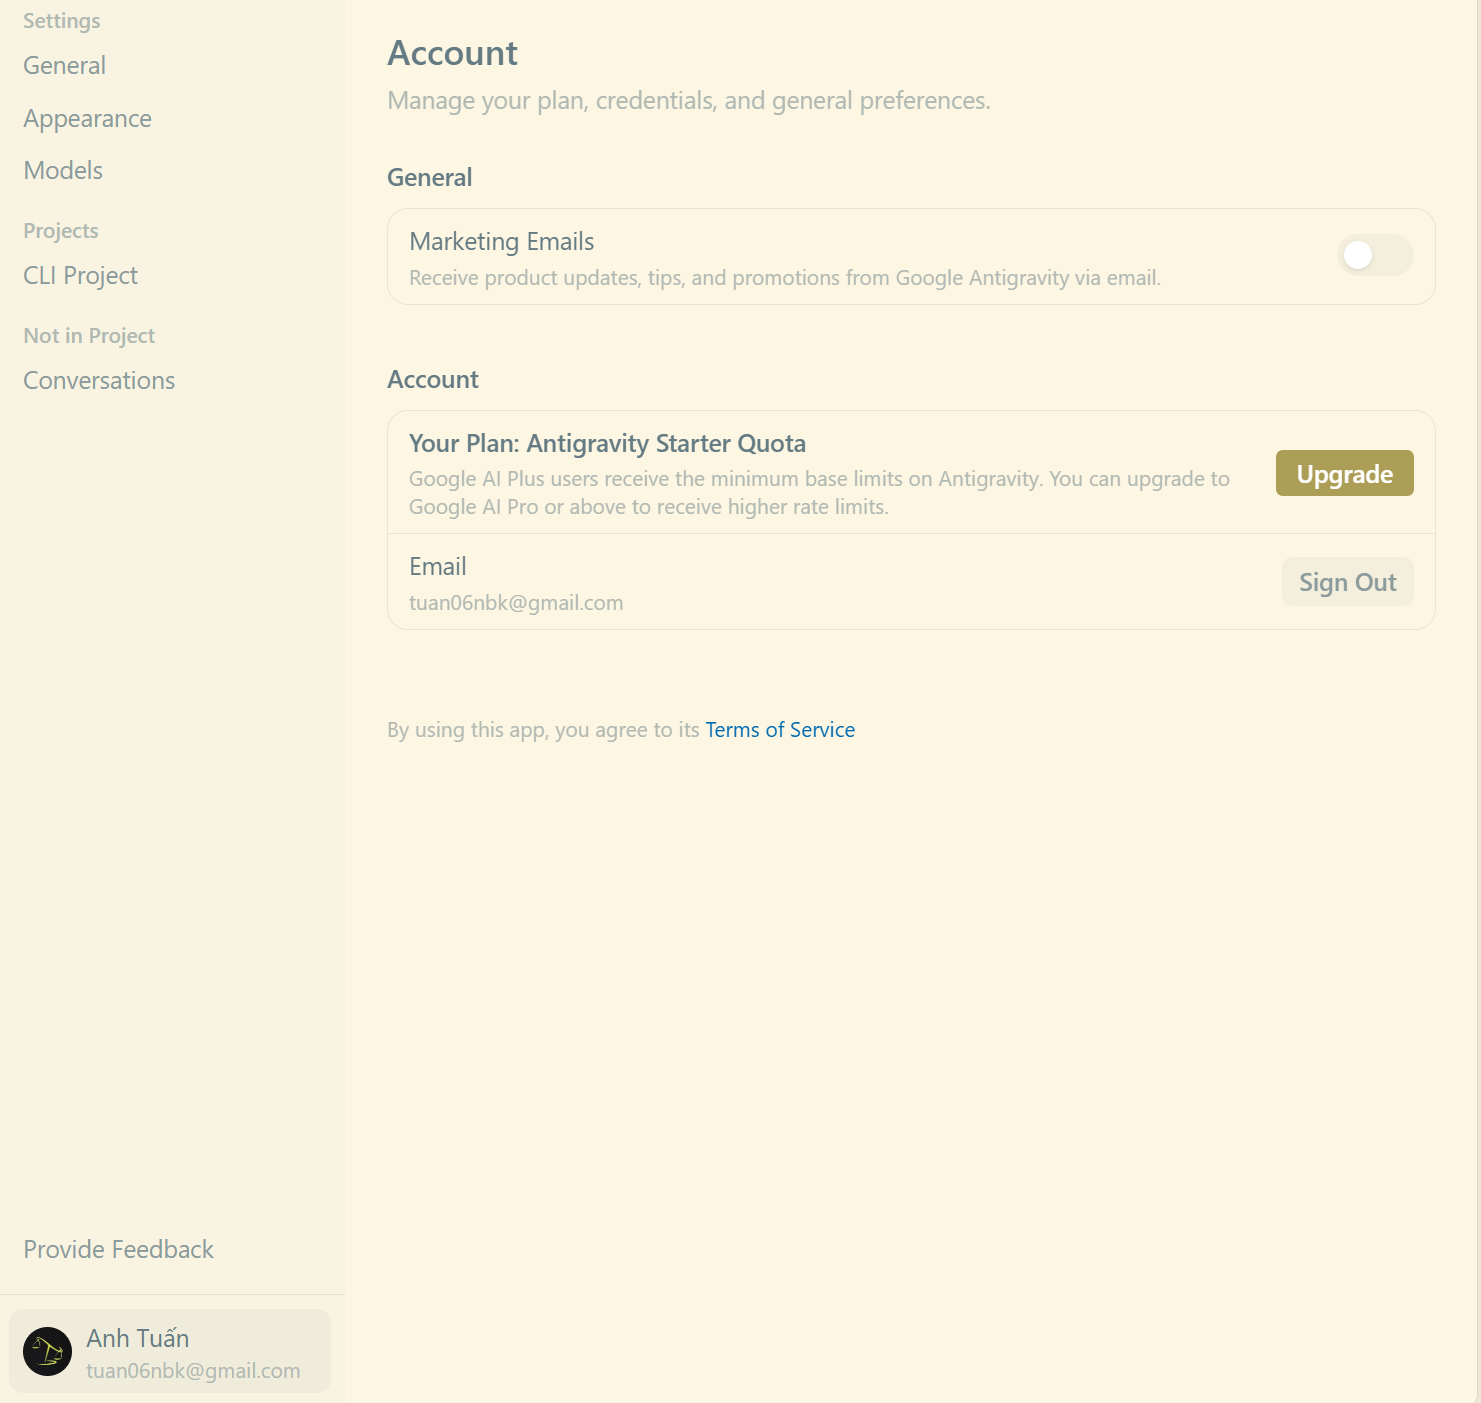
\includegraphics[width=\linewidth]{screenshot/AI_coding_accounts/24125048.png}
        \caption{24125048}
    \end{subfigure}
    \hfill
    \begin{subfigure}{0.3\textwidth}
        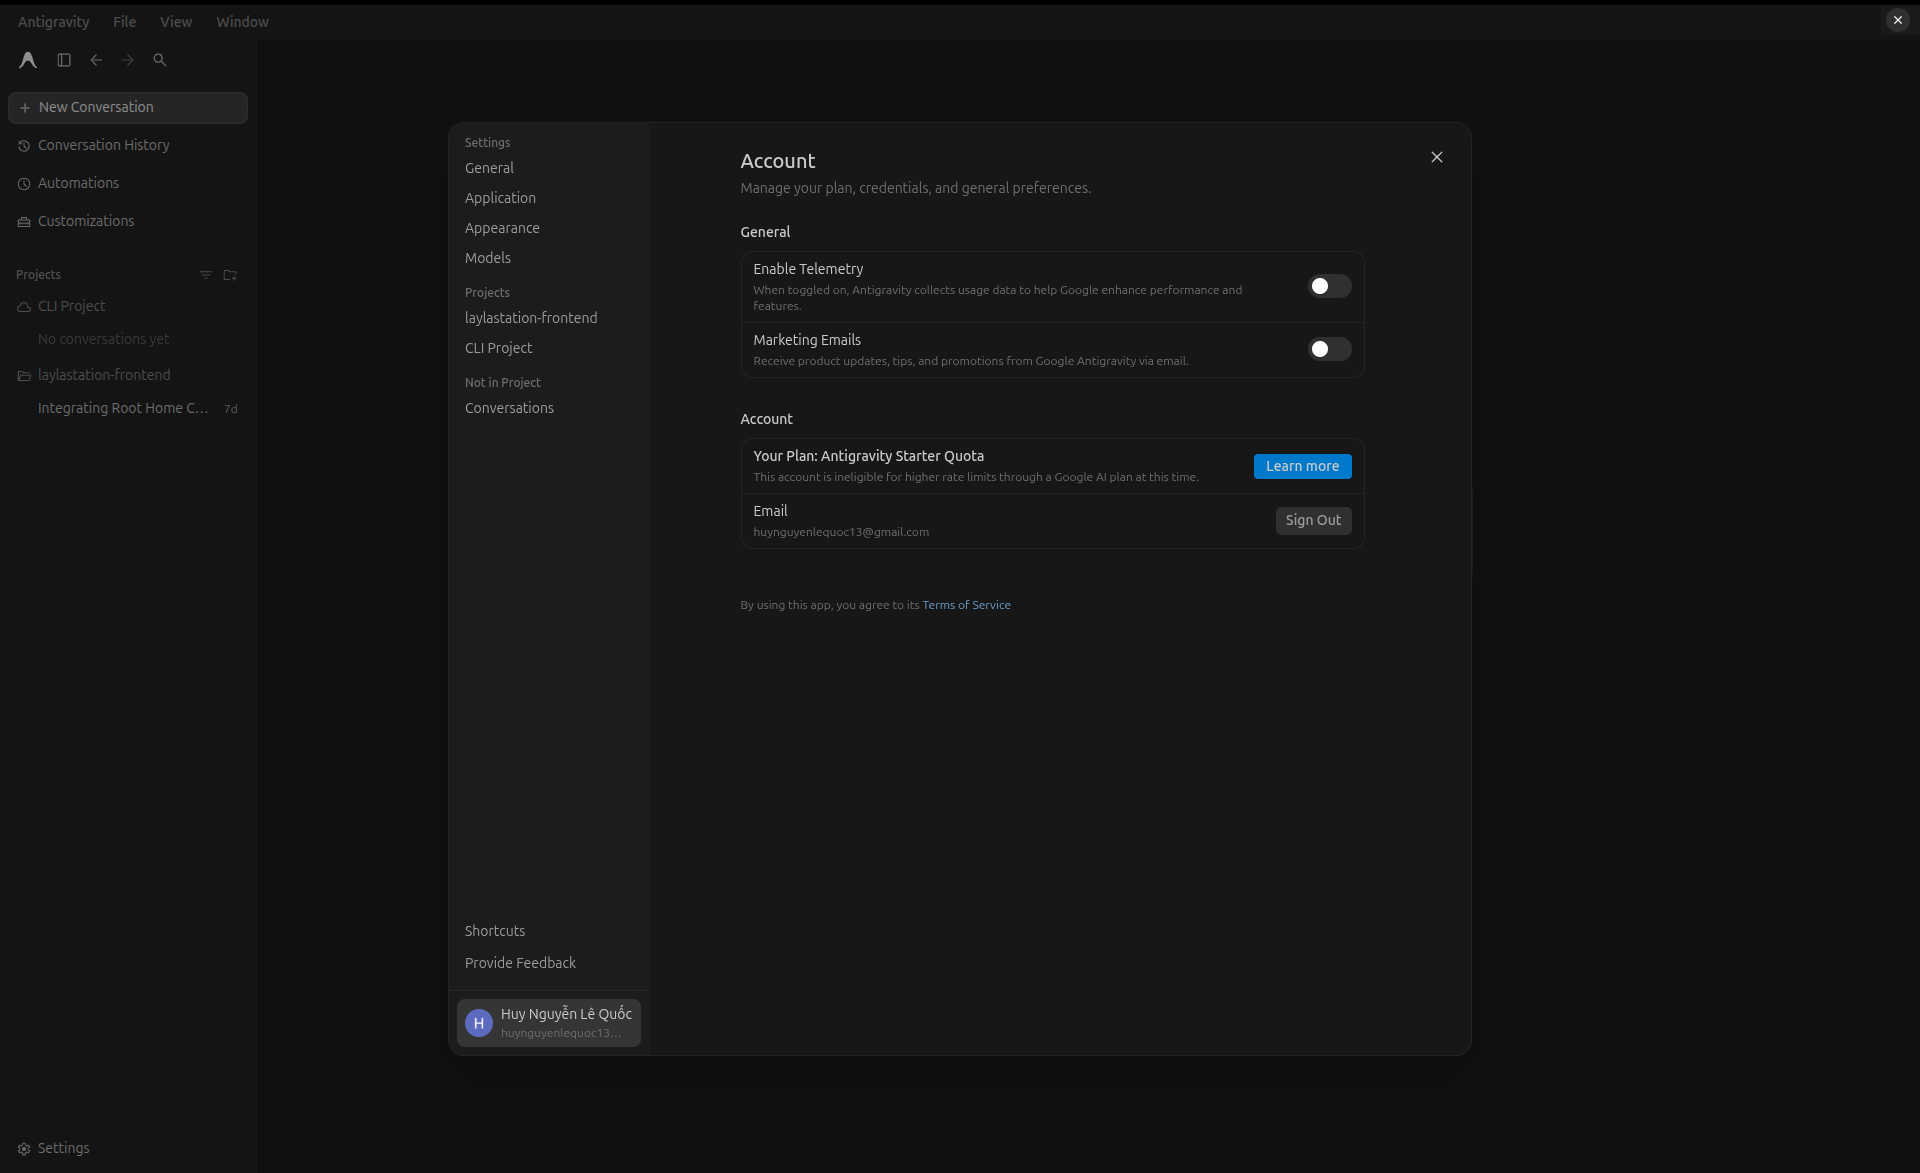
\includegraphics[width=\linewidth]{screenshot/AI_coding_accounts/24125100.png}
        \caption{24125100}
    \end{subfigure}
    \hfill

\end{figure}
\end{document}
